\documentclass[11pt, aspectratio=169]{beamer}
\newcommand{\Set}[2]{\left\{ #1 \;\middle\vert\; #2 \right\}}

\newcommand{\pth}[1]{\mleft(#1\mright)}%

\renewcommand{\P}{\operatorname{P}}
\newcommand{\E}{\operatorname{E}}
\newcommand{\Var}{\operatorname{Var}}
\newcommand{\Cov}{\operatorname{Cov}}
\newcommand{\diam}[1]{\operatorname{diam}\mleft(#1\mright)}
\newcommand{\osc}[2]{\operatorname{osc}\mleft(#1,\, #2\mright)}
\newcommand{\supp}[1]{\operatorname{supp}\mleft(#1\mright)}
\newcommand{\indicator}{\mathbf{1}}
\newcommand{\argmin}{\operatorname{argmin}}
\newcommand{\argmax}{\operatorname{argmax}}
\newcommand{\deq}{\stackrel{d}{=}}

\DeclareMathOperator*{\mtimes}{\text{\raisebox{0.25ex}{\scalebox{0.8}{$\bigtimes$}}}}
\DeclareMathOperator*{\motimes}{\text{\raisebox{0.25ex}{\scalebox{0.8}{$\bigotimes$}}}}

\newcommand{\Ex}[1]{\E\mleft[ #1 \mright]}

\newcommand{\ceil}[1]{\mleft\lceil {#1} \mright\rceil}
\newcommand{\floor}[1]{\mleft\lfloor {#1} \mright\rfloor}
\newcommand{\sgn}{\operatorname{sgn}}
\newcommand{\card}{\operatorname{card}}

\newcommand{\brc}[1]{\left\{ {#1} \right\}}
\newcommand{\sbrc}[1]{\left[ {#1} \right]}
\newcommand{\set}[1]{\brc{#1}}%

\newcommand{\abs}[1]{\left\lvert {#1} \right\rvert}%
\newcommand{\norm}[1]{\left\lVert {#1} \right\rVert}
\newcommand{\spanby}{\operatorname{span}}
\newcommand{\esssup}{\operatorname{ess\,sup}}
\newcommand{\inp}[2]{\left\langle {#1},\, {#2} \right\rangle}

\newcommand{\mto}{\overset{m}{\to}}
\newcommand{\wto}{\overset{w}{\to}}
\newcommand{\wstarto}{\overset{w^*}{\to}}
\newcommand{\asto}{\overset{a.s.}{\to}}
\newcommand{\pto}{\overset{p}{\to}}
\newcommand{\dto}{\overset{d}{\to}}
\newcommand{\dsubset}{\overset{d}{\subset}}


\newcommand{\ds}{\displaystyle}%

\newcommand{\R}{\mathbb{R}}%
\newcommand{\N}{\mathbb{N}}
\newcommand{\Q}{\mathbb{Q}}
\newcommand{\Z}{\mathbb{Z}}
\newcommand{\C}{\mathbb{C}}
\newcommand{\F}{\mathcal{F}}
\newcommand{\A}{\mathcal{A}}
\newcommand{\B}{\mathcal{B}}
\newcommand{\T}{\mathcal{T}}
\newcommand{\M}{\mathcal{M}}
\newcommand{\V}{\mathcal{V}}
\renewcommand{\L}{\mathcal{L}}
\renewcommand{\S}{\mathcal{S}}
\newcommand{\I}{\mathcal{I}}
\renewcommand{\H}{\mathcal{H}}
\newcommand{\D}{\mathcal{D}}
\newcommand{\U}{\mathcal{U}}
\newcommand{\G}{\mathcal{G}}
\newcommand{\J}{\mathcal{J}}

\newcommand{\one}{\mathbf{1}}

\newcommand{\exist}{\exists\:}
\newcommand{\forany}{\forall\:}
\renewcommand{\ae}{\quad\text{a.e.}}
\newcommand{\Res}{\operatorname{Res}}
\newcommand{\cl}{\operatorname{cl}}

\newcommand{\iidsim}{\overset{iid}{\sim}}
\newcommand{\Poisson}{\text{Poisson}}
\newcommand{\Ber}{\text{Ber}}
\newcommand{\Exp}{\text{Exp}}

\newcommand{\restrict}[1]{\left.\hspace{-0.2em}\right|_{#1}}
\newcommand{\eval}[3]{\left.{#1}\right|_{#2}^{#3}}

% derivatives
\makeatletter
\renewcommand\d[1]{\mspace{6mu}\mathrm{d}#1\@ifnextchar\d{\mspace{-3mu}}{}}
\makeatother
\def\at{
  \left.
  \vphantom{\int}
  \right|
}

\newcommand{\od}[2]{\frac{d{#1}}{d{#2}}}
\newcommand{\odd}[2]{\frac{d^2{#1}}{d{#2}^2}}
\newcommand{\pd}[2]{\frac{\partial{#1}}{\partial{#2}}}
\newcommand{\pdd}[2]{\frac{\partial^2{#1}}{\partial{#2}^2}}
\newcommand{\pdpd}[3]{\frac{\partial^2{#1}}{\partial{#2}\partial{#3}}}

\makeatletter
\newcommand*{\rom}[1]{\expandafter\@slowromancap\romannumeral #1@}
\makeatother

\usetheme[progressbar = none, 
    titleformat = smallcaps, 
    numbering = fraction,
    block = fill,
    background = light,
    ]{metropolis}

\usepackage{booktabs}
\usepackage{threeparttable}
\usepackage{tabularx}

\usepackage{pgfplots}
\usepgfplotslibrary{dateplot}

\usepackage{graphicx}
\usepackage{xspace}
\usepackage{hyperref}
%\usepackage[natbibapa]{apacite}
\usepackage{mleftright}
\usepackage[nameinlink]{cleveref}
\usepackage{amsmath, amssymb, algorithm, algorithmicx, algpseudocode}

\title{Pension Run}

\author{Kai-Jyun Wang}
\date{}

\begin{document}

\maketitle

\begin{frame}{Motivation}
    \begin{itemize}[<+->]
        \item The Labor Insurance in Taiwan offers pension options of a lumpsum 
        payment or a monthly pension. 
        \item Should one choose lumpsum or monthly?
        \item Consider a retiree that 
        \begin{itemize}[<+->]
            \item[-] earns over $45,800$ NTD a month, 
            \item[-] has worked for $30$ years, 
            \item[-] retiring at $65$, 
            \item[-] and lives $12$ years after retirement.   
        \end{itemize}
        \item Lumpsum: $2,061,000$ NTD. 
        \item {\color{red}Monthly: $2,724,504$ NTD}. ($2\%$ annual rate)
    \end{itemize}
\end{frame}

\begin{frame}{Annuitization Puzzle}
    \begin{itemize}[<+->]
        \item Annuities insure against longevity
        risk.
        \item Low voluntary annuity purchases/participation. 
        \item Why aren't annuities more popular?
        \begin{itemize}[<+->]
            \item[-] Adverse selection and actuarially unfavorable prices.
            \item[-] Inflation risk and limited availability of indexed annuities.
            \item[-] Pre-existing annuities from public and defined-benefit pensions.
            \item[-] Bequests. 
            \item[-] Medical-expense shocks and liquidity needs.
            \item[-] Behavioral. 
            \item[-] Exogenous provider-insolvency risk.
        \end{itemize}
        \item \textbf{This paper:} Insolvency is endogenous---annuitization choices
        change the fund's liabilities and its probability of depletion.
    \end{itemize}
\end{frame}

\begin{frame}[label=recipient-fraction]{How many people are choosing monthly?}
    \begin{columns}[c,onlytextwidth]
        \begin{column}{0.73\textwidth}
            \centering
            
\includegraphics[width=\textwidth,height=0.78\textheight,keepaspectratio]{%
                ../figure/recipient_fraction.png}
        \end{column}
        \begin{column}{0.25\textwidth}
            \centering
            \hyperlink{data-reconstruction}{%
                \beamergotobutton{View data explanation}}
        \end{column}
    \end{columns}
\end{frame}

\section{Model}

\begin{frame}{Model Overview}
    \begin{itemize}[<+->]
        \item Continuous time and an infinite horizon.
        \item A continuum of workers chooses once, at retirement age $T$,
        between a lump-sum benefit $\ell$ and a monthly pension $p$.
        \item The pension fund earns a stochastic return and receives payroll
        tax revenue.
        \item Benefits stop when the fund balance reaches zero.
        \item Retirees' choices affect fund outflows and, consequently, the
        value of the monthly pension.
    \end{itemize}
\end{frame}

\begin{frame}[label=population]{Population}
    \begin{itemize}[<+->]
        \item Let $g(t,s)$ denote the population density at age $s$:
        \begin{equation*}
            \frac{\partial g}{\partial t}
            \uncover<+->{=-\underbrace{\frac{\partial g}{\partial s}}_{\text{aging}}}
            \uncover<+->{-\underbrace{m(s)g}_{\text{mortality}}}
            \uncover<+->{, \quad
            g(t, 0) = \underbrace{\int b(s)g(t,s)\,ds}_{\text{birth}}.}
        \end{equation*}
        \item Assumptions: 
        \begin{itemize}[<+->]
            \item[-] Constant fertility rate. 
            \item[-] Exposes to constant mortality rate only after $T_m\leq T$.
            \item[-] Stable nomalized population density. 
        \end{itemize}
        \item In steady state, normalized population density $\hat{g} = g / N_t$, $N_t = \int g(t, s)ds$ satisfies
        \begin{equation*}
            \hat g(s)=
            \begin{cases}
                be^{-ns}, & s<T_m,\\
                be^{-ns}e^{-m(s-T_m)}, & s\geq T_m,
            \end{cases}
        \end{equation*}
        where $dN_t = nN_tdt$ is the population growth rate.
        \hyperlink{population-density}{%
            \beamergotobutton{View population density}}
    \end{itemize}
\end{frame}


\begin{frame}{Retiree Pension Choice}
    \begin{itemize}[<+->]
        \item A retiring individual chooses between lumpsum and monthly to maximize
        \begin{equation*}
            u_{it}(d)=
            \begin{cases}
                \uncover<+->{\alpha+\log(\underbrace{\ell}_{\text{lumpsum}})+\epsilon_i(\ell),}
                & \uncover<.->{d=\text{lumpsum},}\\
                \uncover<+->{\log(\underbrace{V(\hat B_t,\hat Q_t)}_{\text{PDV of monthly}})+\epsilon_i(p),}
                & \uncover<.->{d=\text{pension}.}
            \end{cases}
        \end{equation*}
        \item The PDV of monthly is 
        \begin{equation*}
            V(\hat B,\hat Q)
            =\mathbb E\left[\left.\int_0^{T_{\hat B}}
            e^{-(\rho+m)s}\underbrace{p}_{\text{monthly benefit}}\,ds\,\right|\,\hat B,\hat Q\right]
        \end{equation*}
        where $T_{\hat{B}}$ is the bankruptcy time.
    \end{itemize}
\end{frame}

\begin{frame}{Pension System}
    \begin{itemize}[<+->]
        \item Monthly recipients $Q_t$:
        \begin{equation*}
            dQ_t=\big[
            \uncover<+->{\underbrace{q_t\hat g(T)N_t}_{\text{new retirees}}}
            \uncover<+->{-\underbrace{mQ_t}_{\text{mortality}}}\big]dt.
        \end{equation*}
        \item $q_t$: share of monthly among new retirees.
        \item Fund balance $B_t$: 
        \begin{align*}
            dB_t={}&\big[
            \uncover<+->{\underbrace{rB_t}_{\text{return}}}
            \uncover<+->{+\underbrace{\tau yN_t\int_{T_w}^{T}\hat g(s)\,ds}_{\text{pension tax}}}
            \uncover<+->{-\underbrace{\ell(1-q_t) N_t\hat g(T)}_{\text{lump sum}}}
            \uncover<+->{-\underbrace{pQ_t}_{\text{monthly}}}\big]dt
            \uncover<+->{+\underbrace{\sigma B_t\,dZ_t}_{\text{stochastic}}}.
        \end{align*}
    \end{itemize}
\end{frame}

\begin{frame}{Detrended State Dynamics}
    \begin{itemize}[<+->]
        \item Define per capita states
        $\hat B_t=B_t/N_t$ and $\hat Q_t=Q_t/N_t$.
        \begin{align*}
            d\hat B_t={}&\big[
            \underbrace{(r-n)\hat B_t}_{\text{net return}}
            +\underbrace{\tau y\int_{T_w}^{T}\hat g(s)\,ds}_{\text{pension tax}}
            -\underbrace{\ell(1-q_t)\hat g(T)}_{\text{lump sum}}
            -\underbrace{p\hat Q_t}_{\text{monthly}}\big]dt
            +\underbrace{\sigma\hat B_t\,dZ_t}_{\text{stochastic}},\\
            d\hat Q_t={}&\big[
            \underbrace{q_t\hat g(T)}_{\text{new retirees}}
            -\underbrace{(m+n)\hat Q_t}_{\text{mortality}}\big]dt.
        \end{align*}
        \item More lump-sum claims reduce the fund immediately.
        \item More monthly claims raise future liabilities through $\hat Q_t$.
    \end{itemize}
\end{frame}

\begin{frame}{Aggregation and Equilibrium}
    \begin{itemize}[<+->]
        \item Assume the idiosyncratic preference $\epsilon_{it}(d)\sim \text{Gumbel}(0, 1)$. 
        \begin{equation*}
            q_t = q(\hat{B}_t, \hat{Q}_t) = \frac{1}{1+\exp\big(\alpha+\log(\underbrace{\ell}_{\text{lumpsum}})-\log(\underbrace{V(\hat B_t,\hat Q_t)}_{\text{PDV of monthly}})\big)}
        \end{equation*}
        \item In equilibrium: 
        \begin{itemize}[<+->]
            \item[-] Given belief on $T_{\hat{B}}$, new retirees choose between lumpsum and monthly optimally. 
            \item[-] Individuals optimizing aggregates up to $q_t$.  
            \item[-] $q_t$ implies the state dynamics consistent with the belief on $T_{\hat{B}}$.
        \end{itemize}
    \end{itemize}
    
\end{frame}

\begin{frame}[label=numerical-solution]{Value Function and Numerical Solution}
    \begin{itemize}[<+->]
        \item The PDV of monthly solves the nonlinear HJB equation
        \begin{equation*}
            \begin{split}
                (\rho+m)V(\hat{B}, \hat{Q})&=\uncover<+->{\underbrace{p}_{\text{monthly benefit}}}\\ 
                &\uncover<+->{+\underbrace{\big[(r-n)\hat B_t
                +\tau y\int_{T_w}^{T}\hat g(s)\,ds
                -\ell(1-q_t)\hat g(T)
                -p\hat Q_t\big]}_{\text{drift of $\hat{B}$}}\pd{V}{\hat{B}}} \\ 
                &\uncover<+->{+\underbrace{\big[q_t\hat g(T)-(m+n)\hat Q_t\big]}_{\text{drift of $\hat{Q}$}}\pd{V}{\hat{Q}}}
                \uncover<+->{+ \frac{1}{2}(\underbrace{\sigma \hat{B}_t}_{\text{diffusion of $\hat{B}$}})^2\pdd{V}{\hat{B}}}
            \end{split}
        \end{equation*}
        \item Boundary condition: $V(0, \hat{Q}) = 0$. 
        \item At a sufficiently large upper boundary, impose
        $\partial V/\partial\hat B\approx0$.
        \item Solve by finite differences and successive iteration, 
        equivalent to semi-implicit scheme with $dt = \infty$. 
        \hyperlink{numerical-algorithm}{%
        \beamergotobutton{View algorithm}}
    \end{itemize}
\end{frame}

\section{Results}

\begin{frame}{Calibration}
    \footnotesize
    \setlength{\tabcolsep}{3pt}
    \renewcommand{\arraystretch}{0.92}
    \begin{table}[t]
        \begin{threeparttable}
    \begin{tabular}{clcl}
        \toprule
        Parameter & Description & Value & Target \\
        \midrule
        \multicolumn{4}{l}{\textit{Panel A: External Calibration}} \\
        \addlinespace
        $b$ & Birth rate & $0.00462$ & Total fertility rate \\
        $m$ & Mortality rate & $0.06$ & Median lifespan \\
        $T_w$ & Working age & $25$ &  \\
        $T_r$ & Retirement age & $61$ & Standard retirement age \\
        $T_m$ & Age of mortality exposure & $60$ &  \\
        $\rho$ & Subjective discount rate & $0.02$ & Interest rate \\
        $\tau$ & Pension tax & $0.075$ & Pension tax \\
        $y$ & Income & $5.268$ & Highest monthly insured salary \\
        $\ell$ & Lump-sum pension & $19.75$ & Transfer based on 30 years of working \\
        $p$ & Monthly pension & $2.449$ & Pension based on 30 years of working \\
        \bottomrule
    \end{tabular}

    \begin{tablenotes}[flushleft]
        \footnotesize
        \item \textit{Note:} The monetary unit in the model is 100,000 NTD.
    \end{tablenotes}
\end{threeparttable}

    \end{table}
\end{frame}

\begin{frame}{Calibration}
    \footnotesize
    \setlength{\tabcolsep}{3pt}
    \renewcommand{\arraystretch}{1.05}
    \begin{table}[t]
        \begin{threeparttable}
    \begin{tabular}{clcl}
        \toprule
        Parameter & Description & Value & Target \\
        \midrule
        \multicolumn{4}{l}{\textit{Panel B: Internal Calibration}} \\
        \addlinespace
        $r$ & Pension fund return rate & $0.2686$ & $\E\sbrc{\frac{\hat{B}_{t+\Delta}-\hat{B}_t}{B_t}-\mu_{B}(\hat{B}_t, \hat{Q}_t, \theta)\Delta} = 0$ \\
        $\sigma$ & Pension fund volatility & $1.855$ & $\text{SD}(\frac{\hat{B}_{t+\Delta}-\hat{B}_t}{B_t\sqrt{\Delta}}) = \sigma$ \\
        $\alpha$ & Preference for lump-sum scheme & $-17.43$ & $\E\sbrc{(q - q(\hat{B}_t, \hat{Q}_t, \theta))^2}$ \\
        $\beta$ & Sensitivity to default risk & $0.6663$ & $\E\sbrc{(q - q(\hat{B}_t, \hat{Q}_t, \theta))^2}$ \\
        \bottomrule
    \end{tabular}

    \begin{tablenotes}[flushleft]
        \footnotesize
        \item \textit{Note:} The monetary unit in the model is 100,000 NTD.
    \end{tablenotes}
\end{threeparttable}

    \end{table}
\end{frame}

\begin{frame}{Estimated $V$}
    \centering
    \only<1>{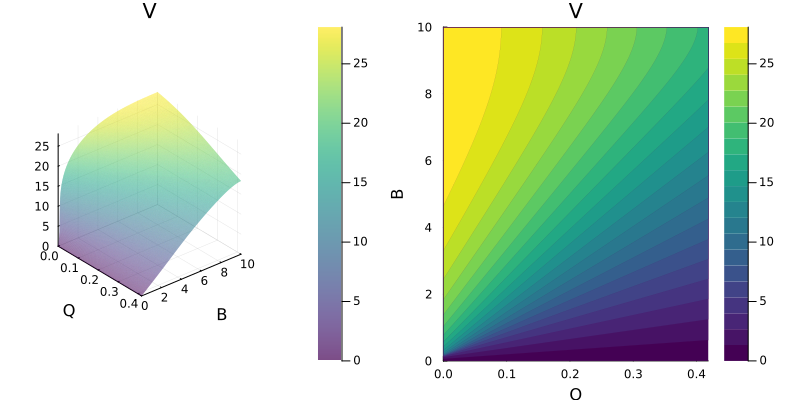
\includegraphics[scale=0.5]{../figure/estimated_V.png}}
    \only<2>{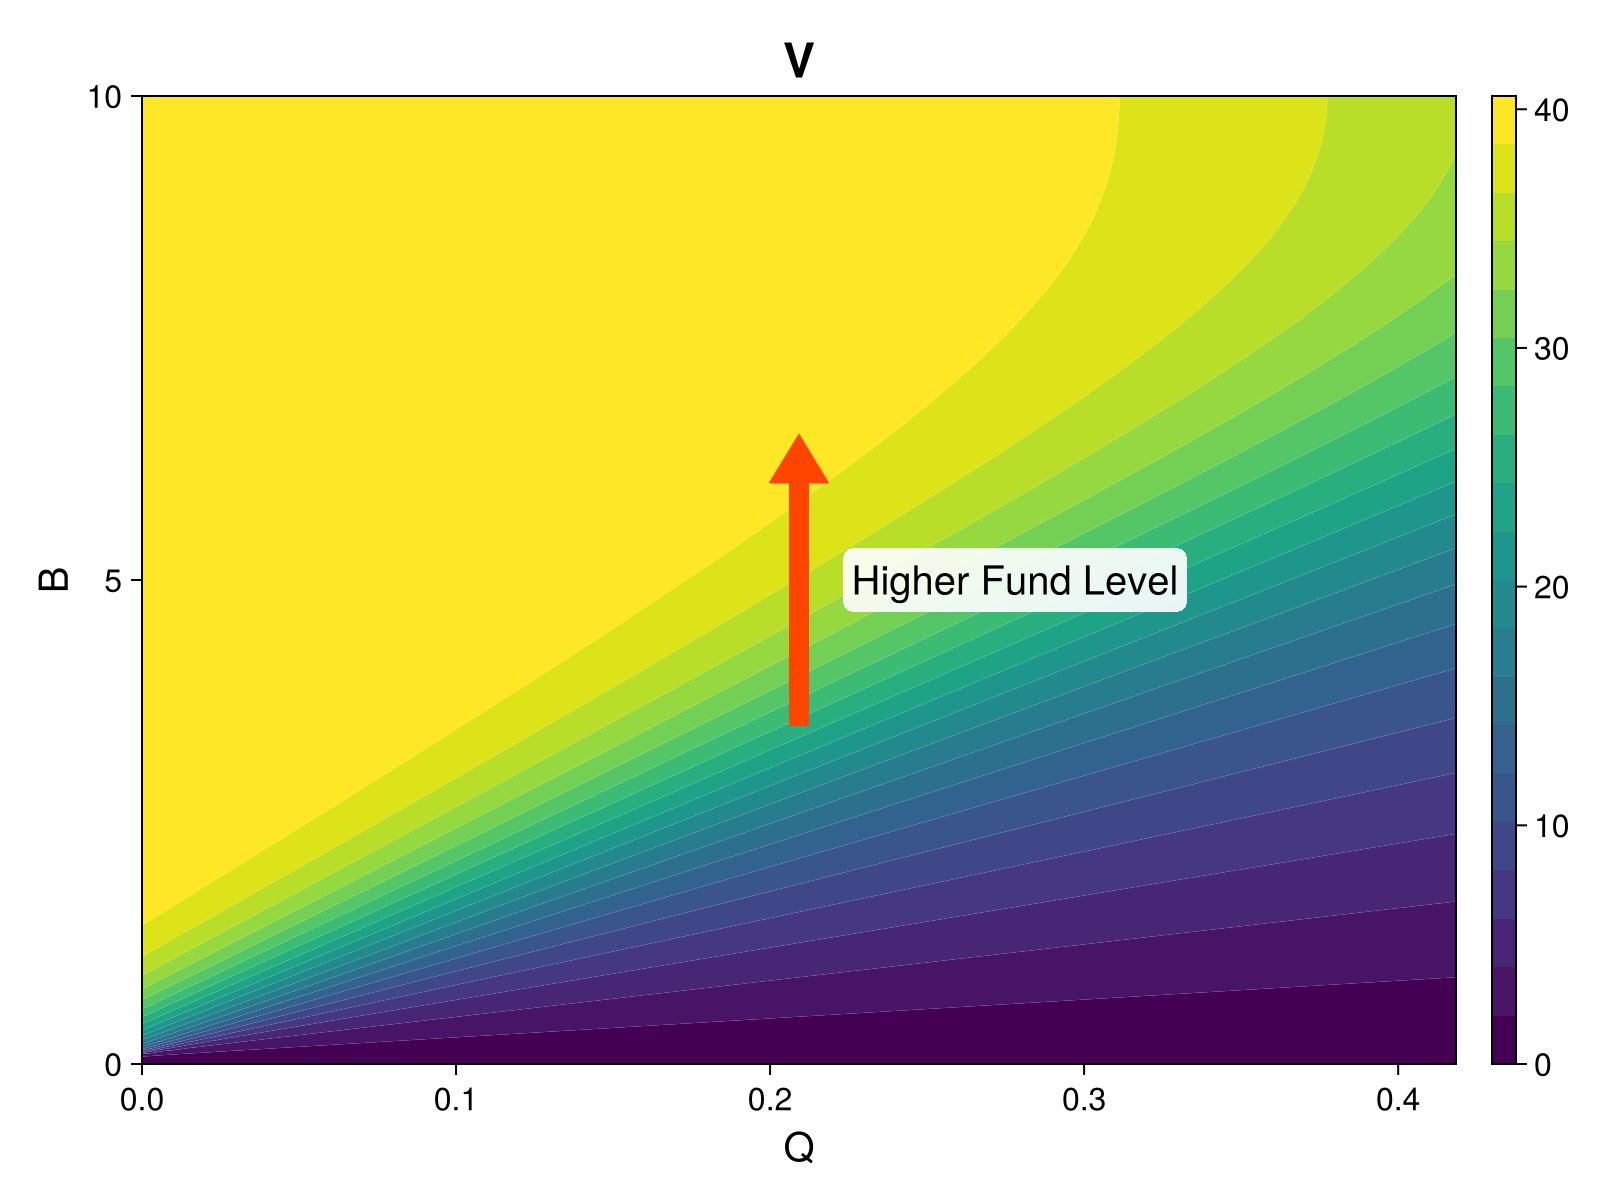
\includegraphics[scale=0.5]{../figure/estimated_V_higher_fund.png}}
    \only<3>{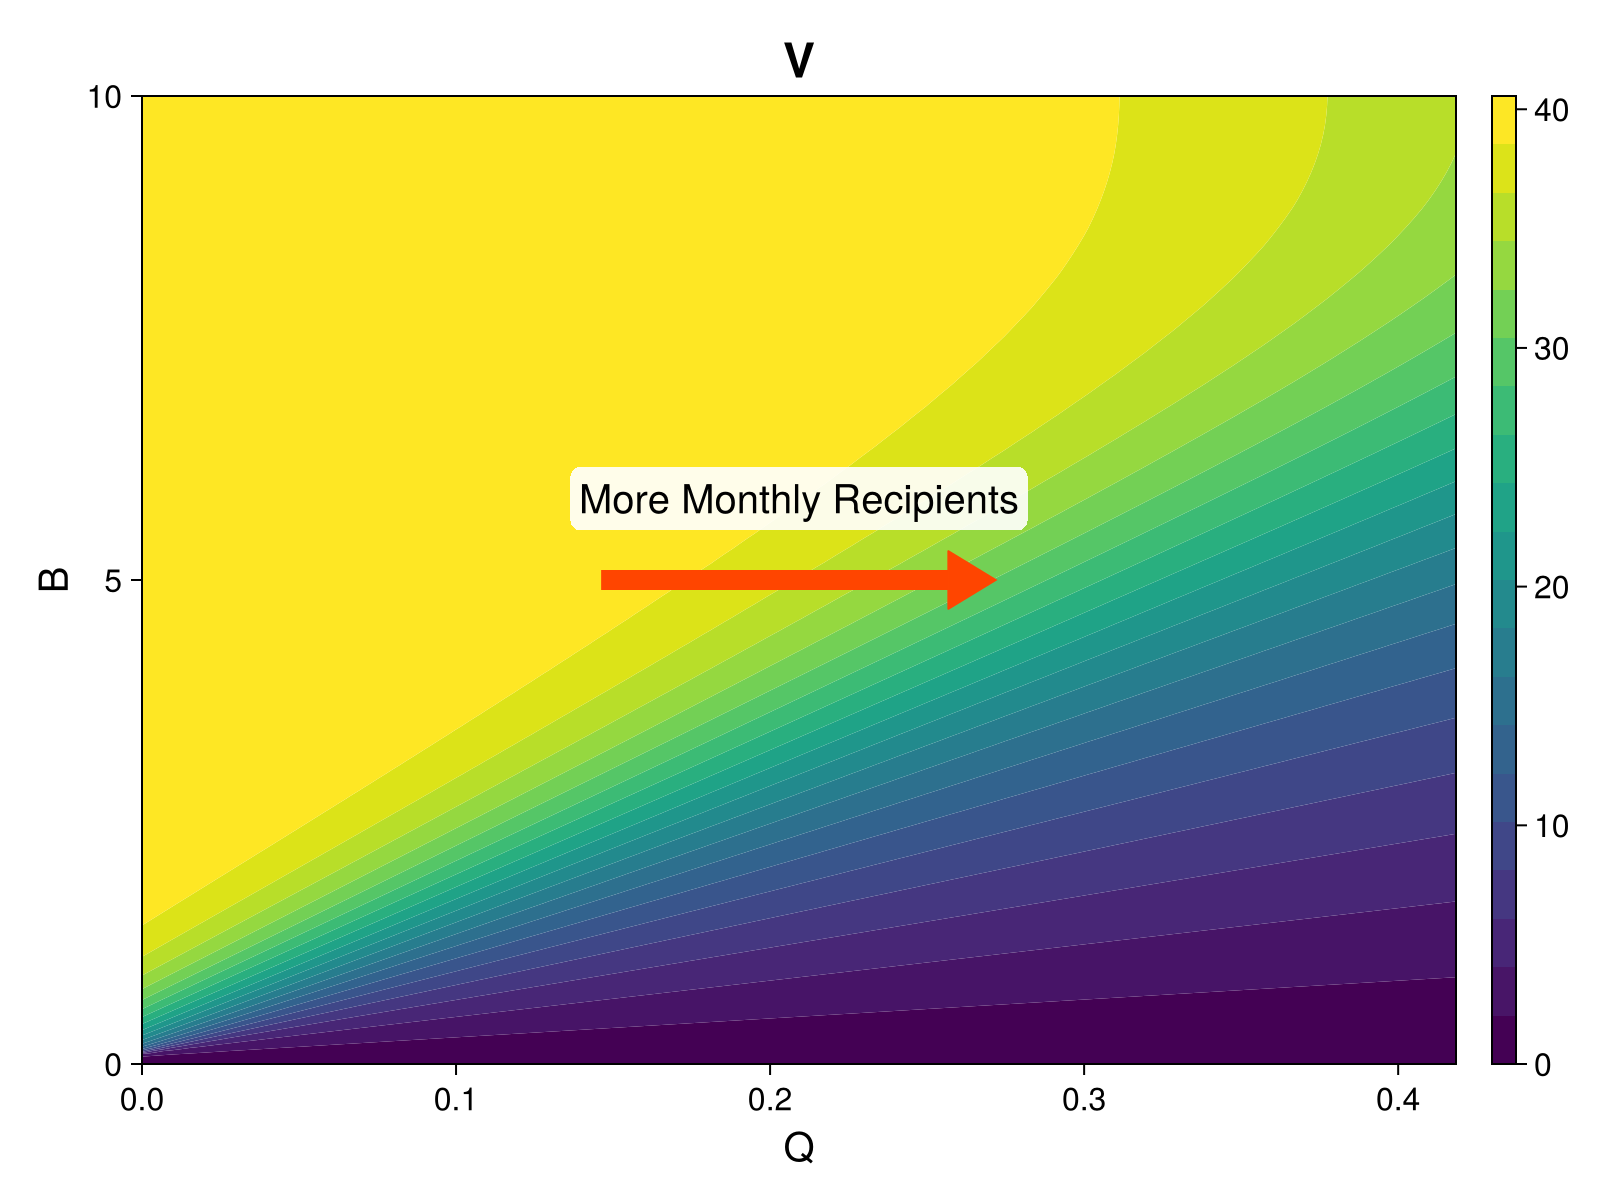
\includegraphics[scale=0.5]{../figure/estimated_V_more_monthly_recipients.png}}
\end{frame}

\begin{frame}{Model Fit}
    \centering
    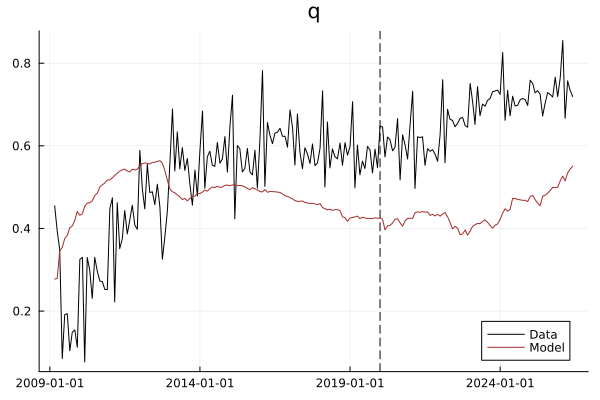
\includegraphics[scale=0.5]{../figure/validation_q.png}
\end{frame}

\begin{frame}{Low Pension Tax Rate}
    \centering
    \only<1>{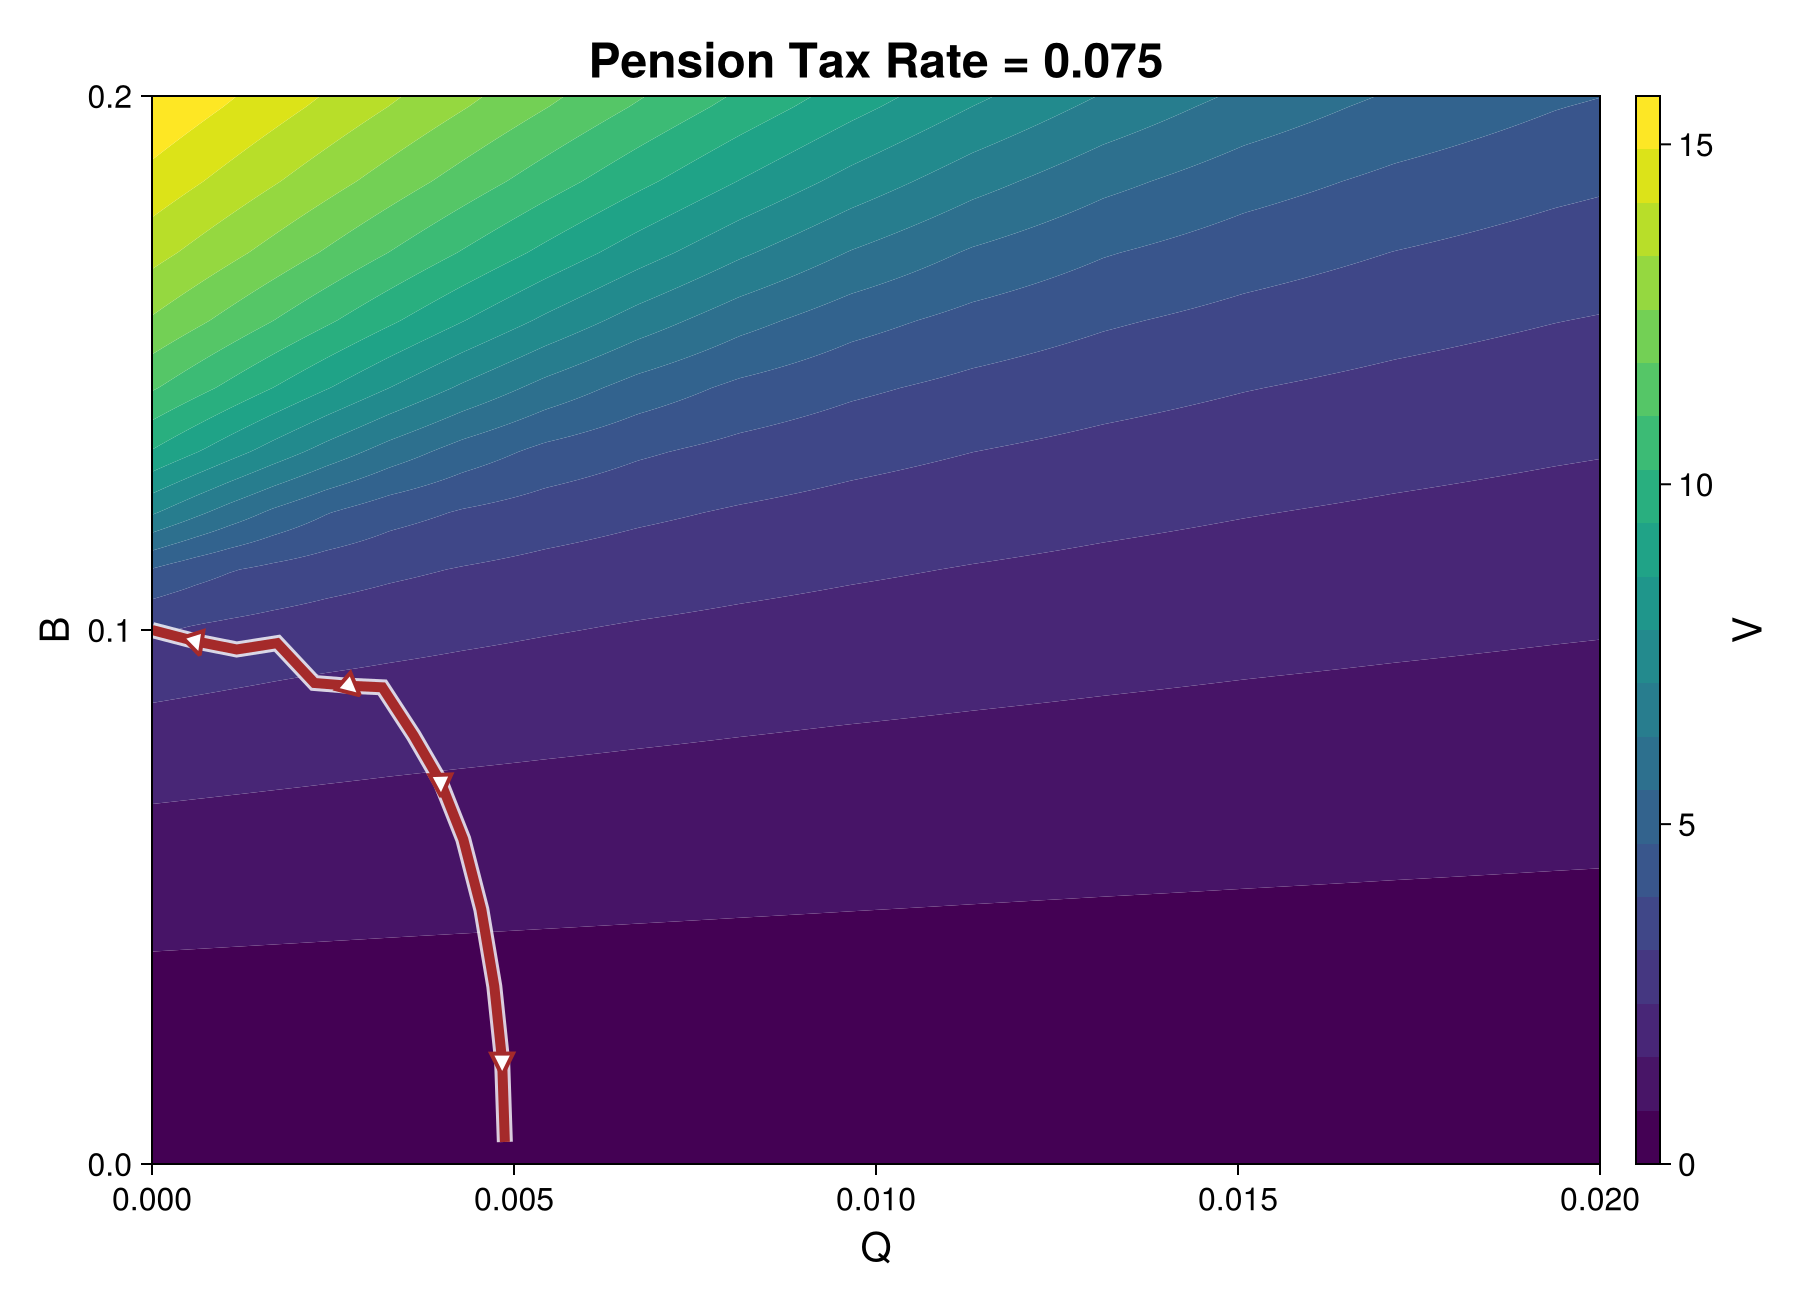
\includegraphics[scale=0.45]{../figure/mechanism_tax_0075_stage_0_trajectory.png}}
    \only<2>{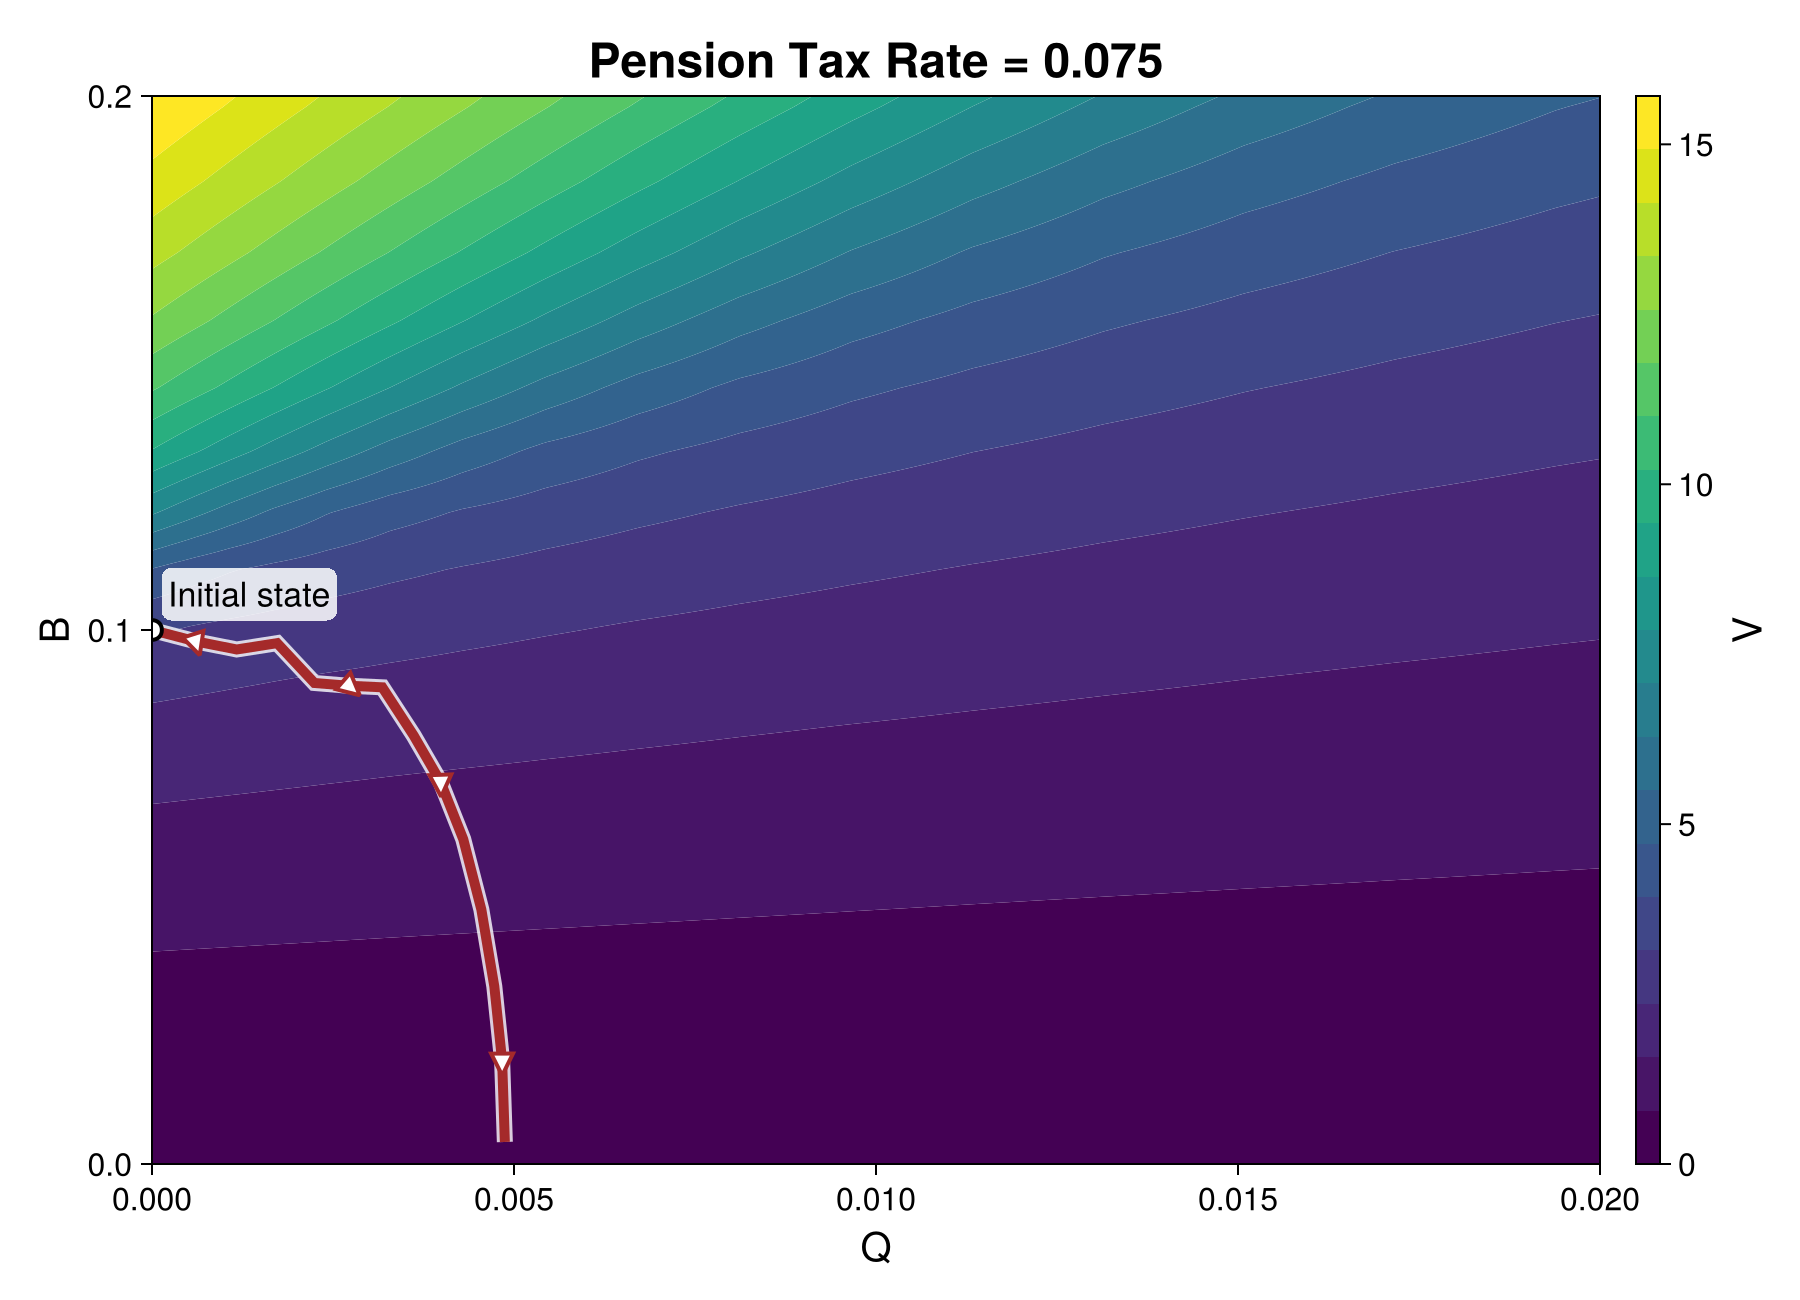
\includegraphics[scale=0.45]{../figure/mechanism_tax_0075_stage_1_initial_state.png}}
    \only<3>{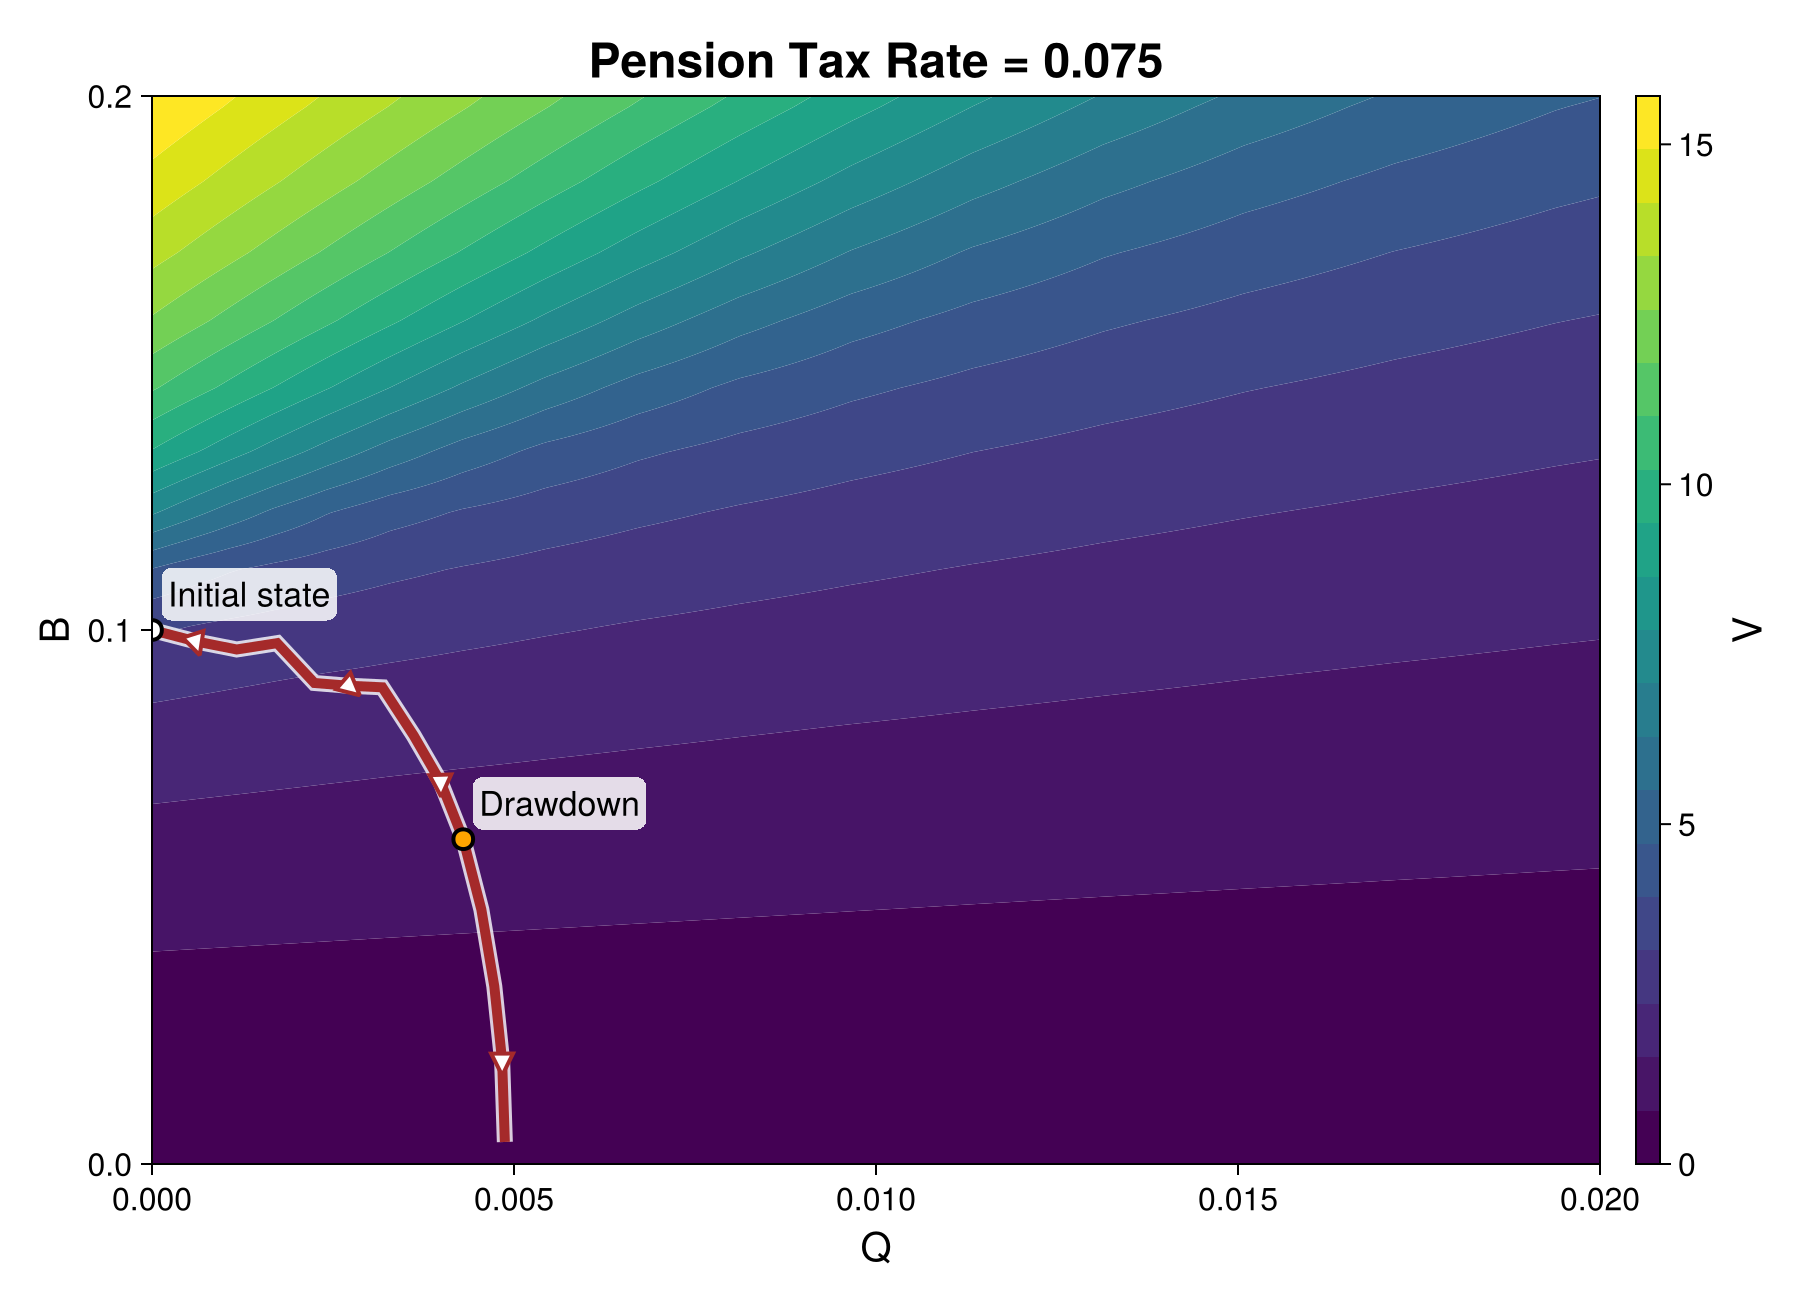
\includegraphics[scale=0.45]{../figure/mechanism_tax_0075_stage_2_drawdown.png}}
    \only<4>{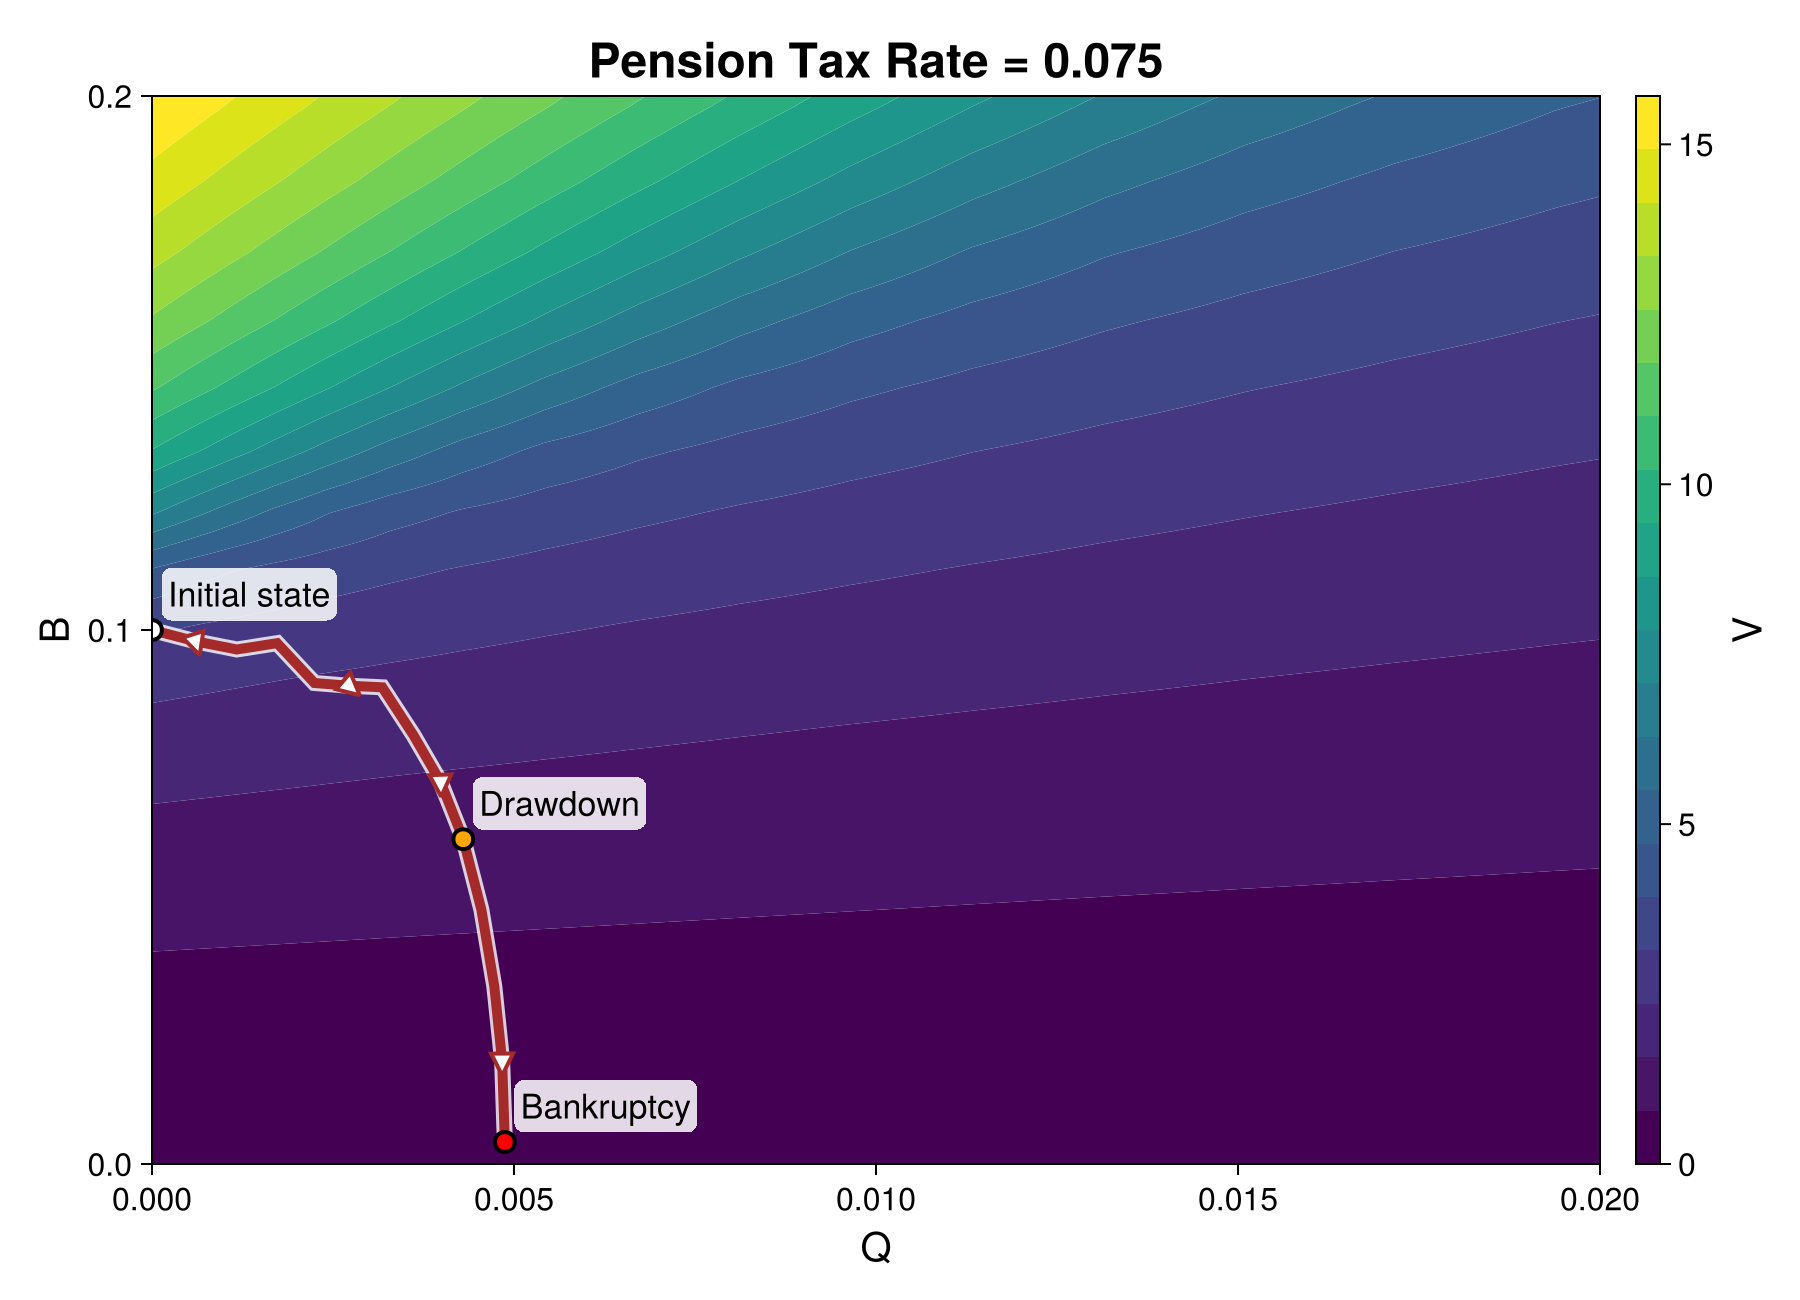
\includegraphics[scale=0.45]{../figure/mechanism_tax_0075_stage_3_bankruptcy.png}}
\end{frame}

\begin{frame}{Medium Pension Tax Rate}
    \centering
    \only<1>{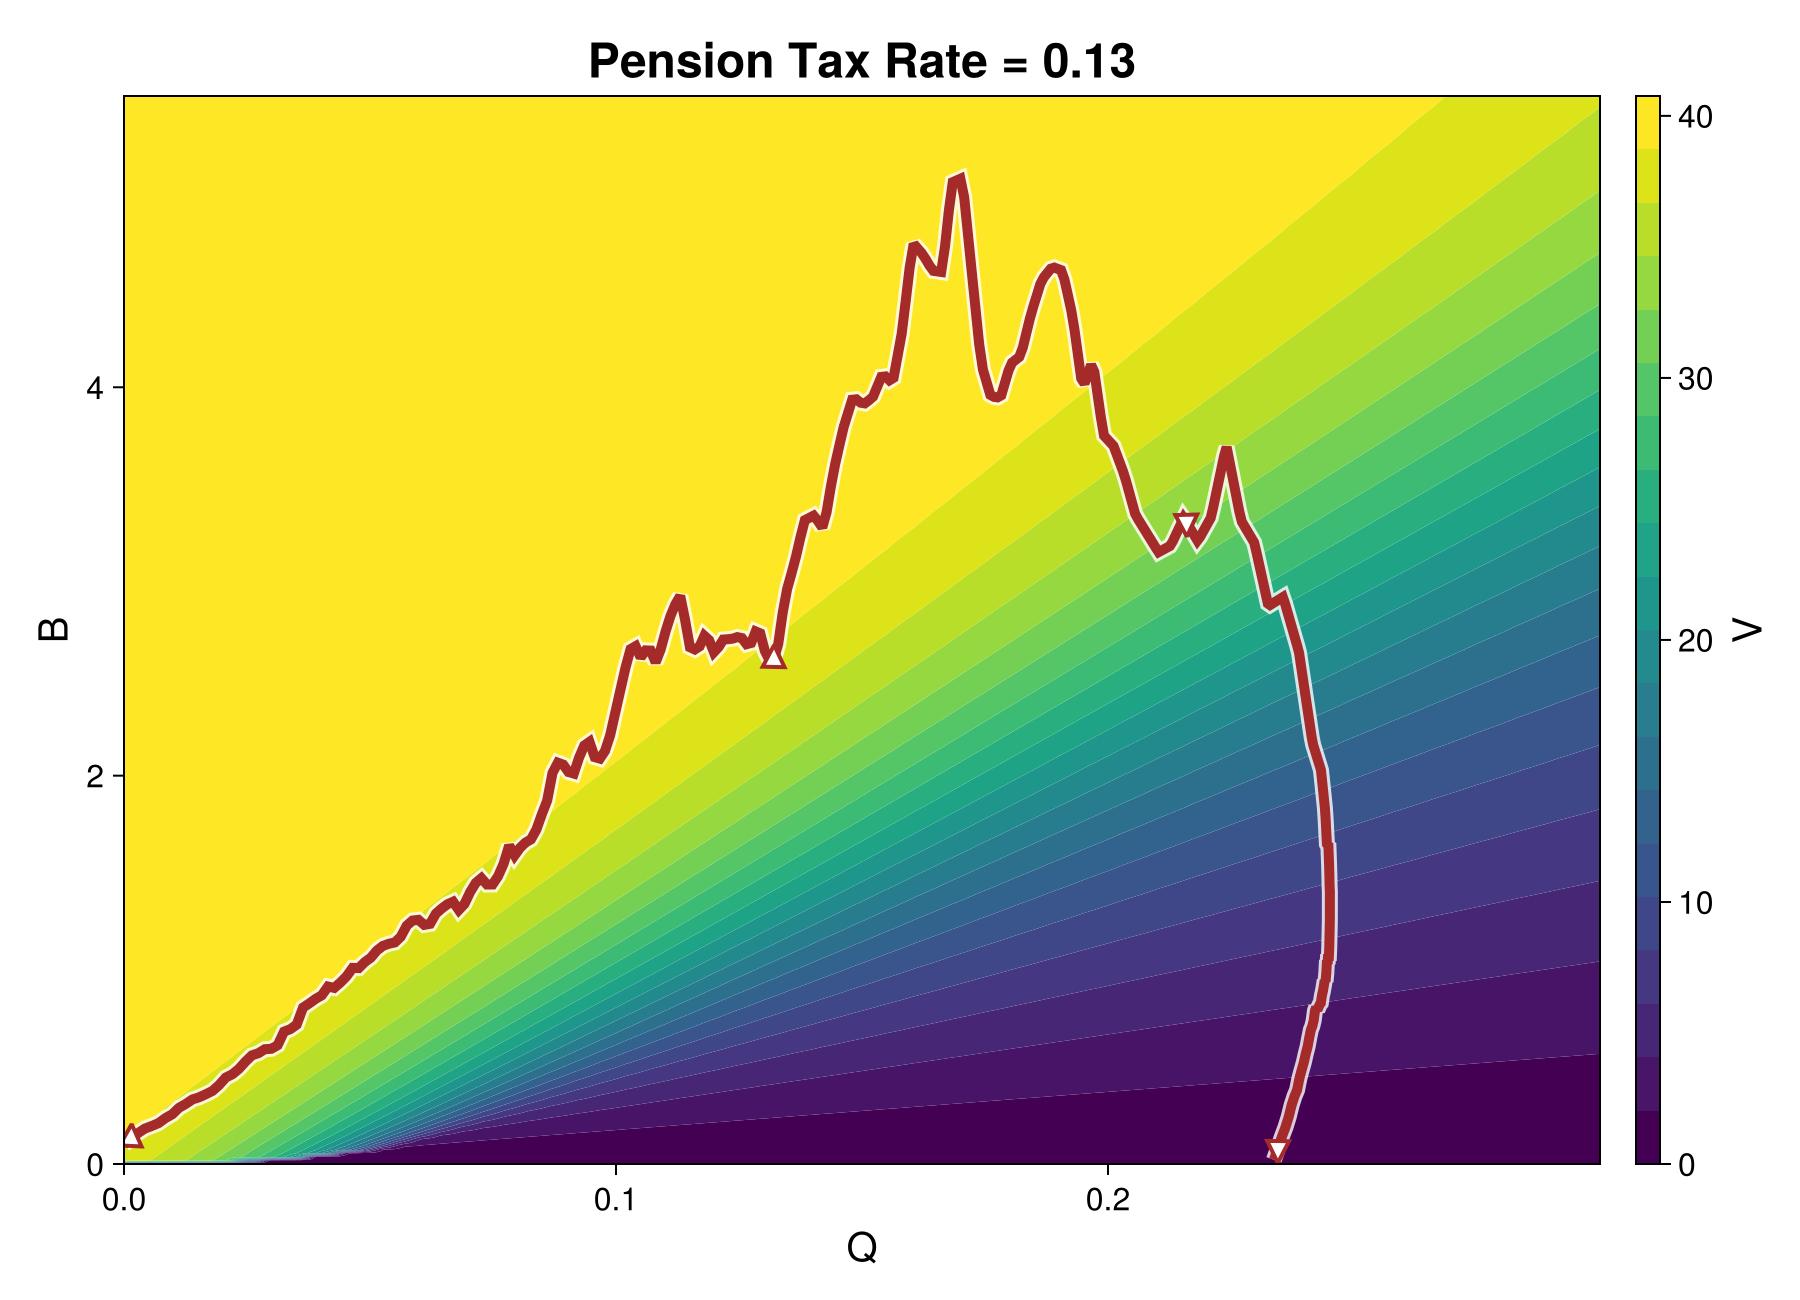
\includegraphics[scale=0.45]{../figure/mechanism_tax_013_stage_0_trajectory.png}}
    \only<2>{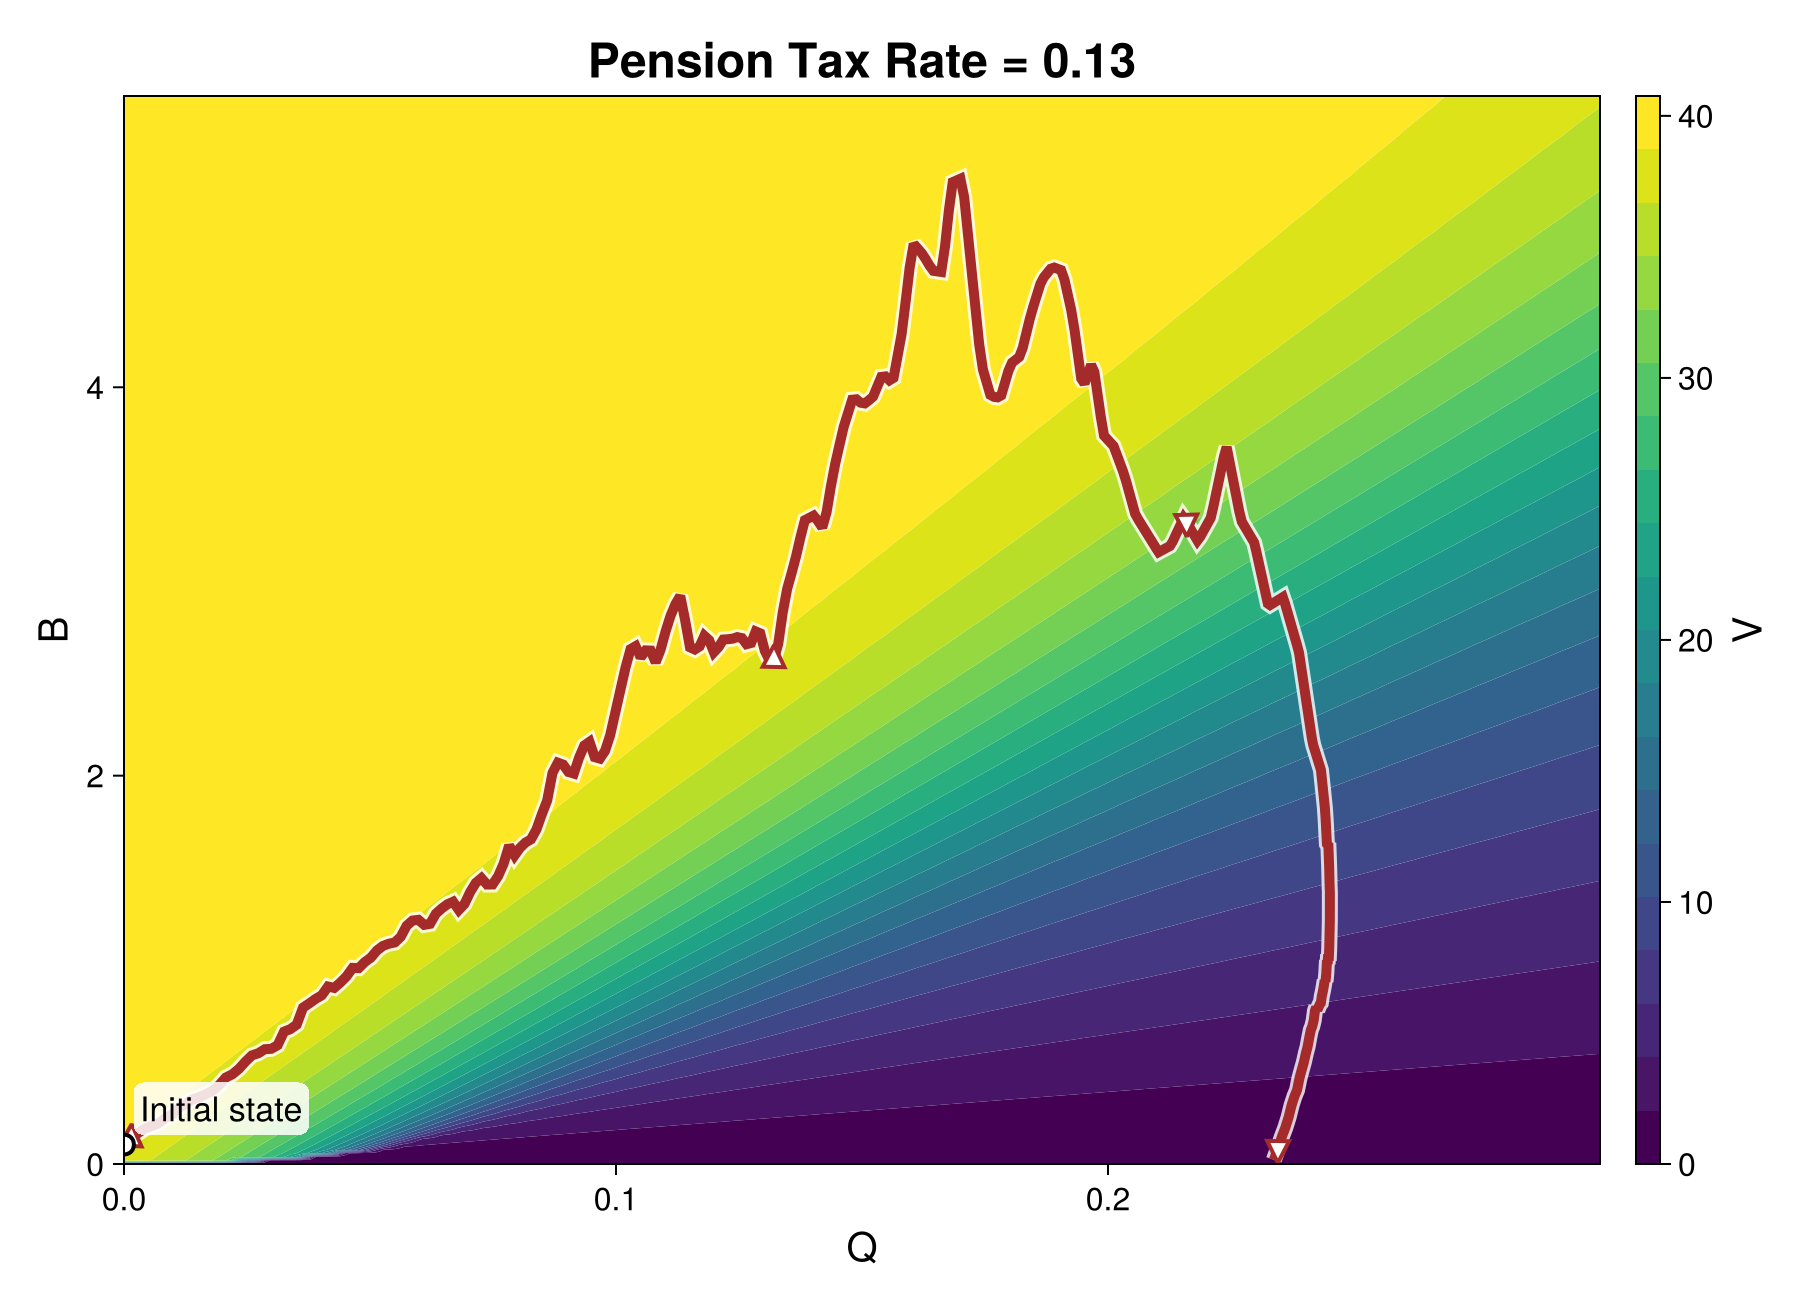
\includegraphics[scale=0.45]{../figure/mechanism_tax_013_stage_1_initial_state.png}}
    \only<3>{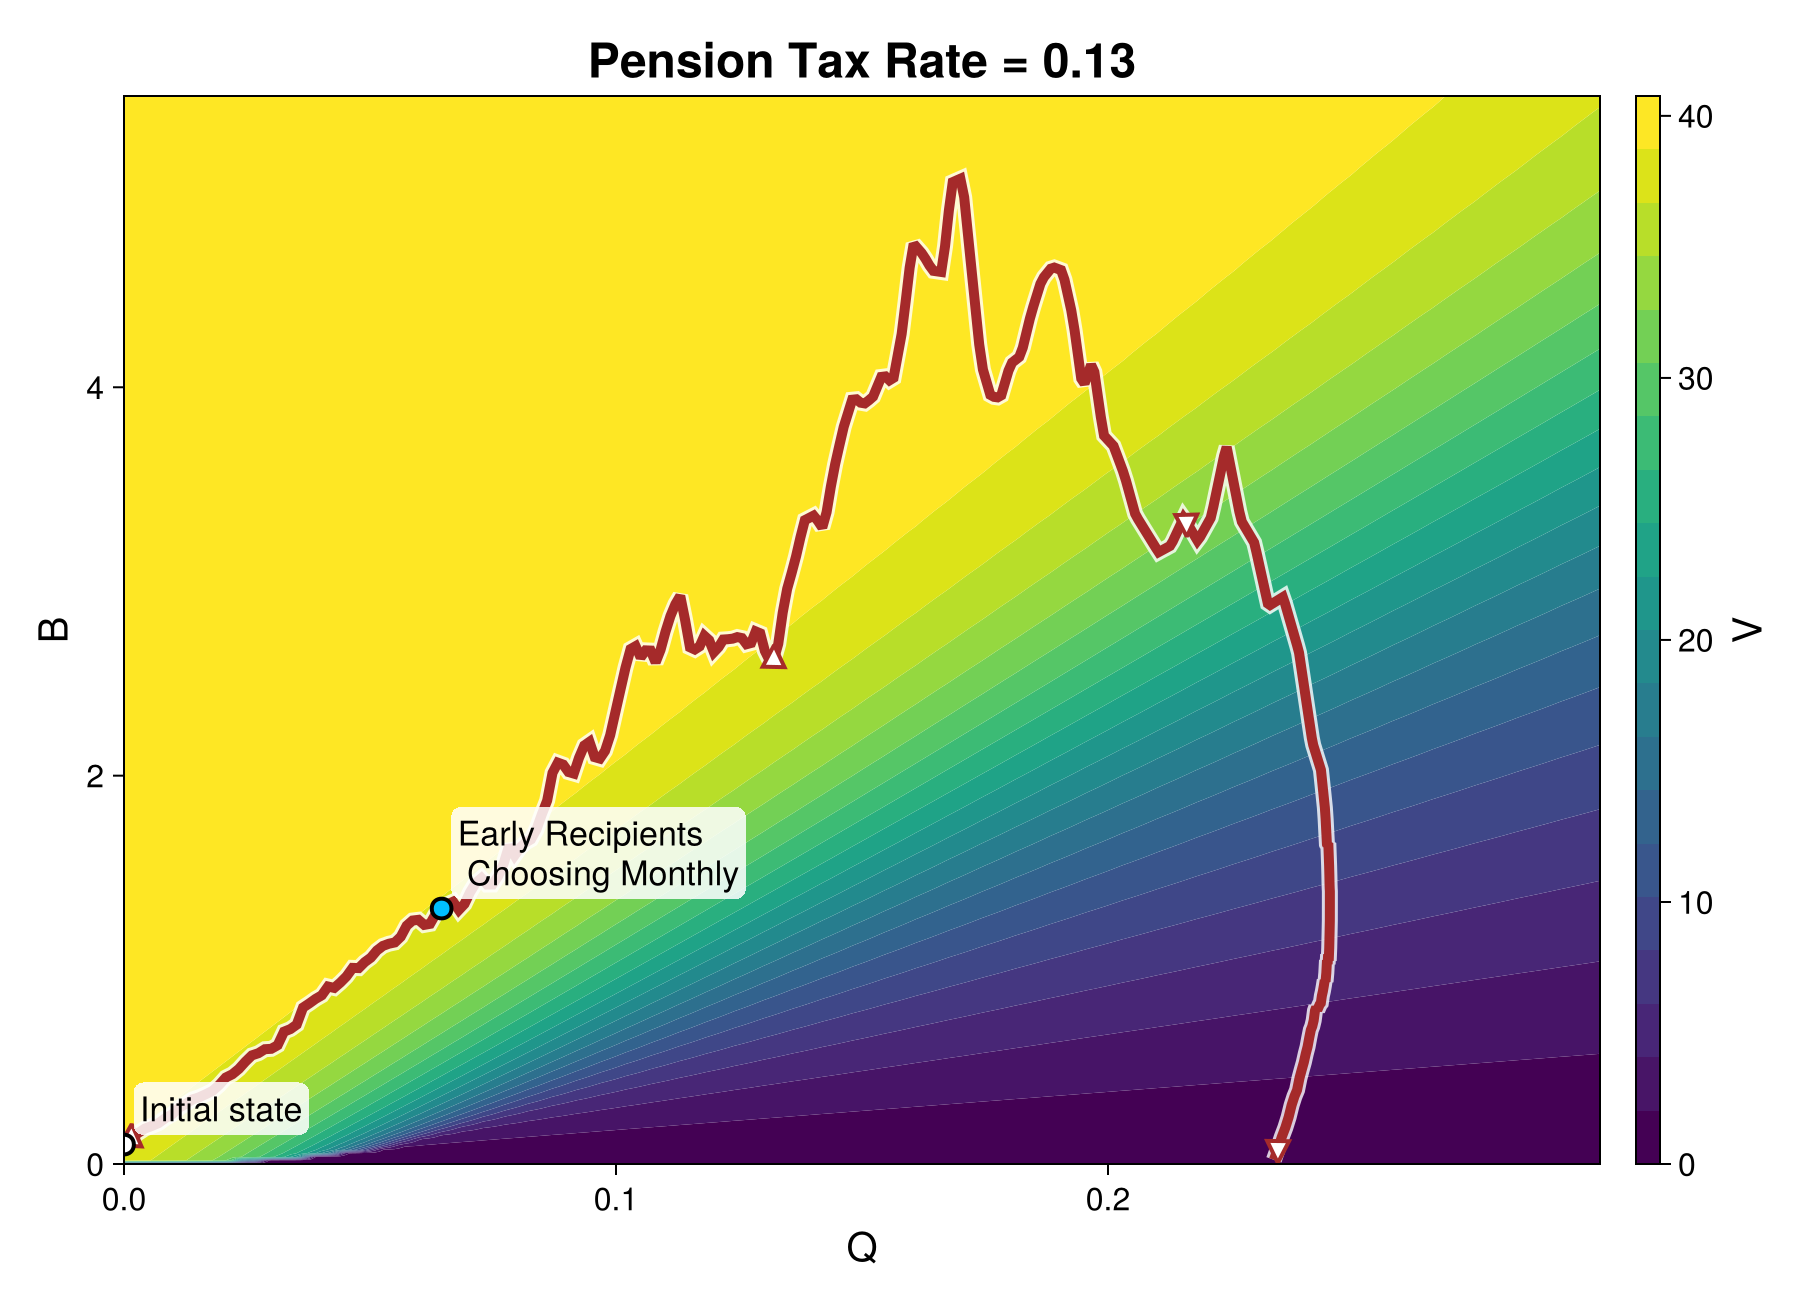
\includegraphics[scale=0.45]{../figure/mechanism_tax_013_stage_2_early_recipients_choosing_monthly.png}}
    \only<4>{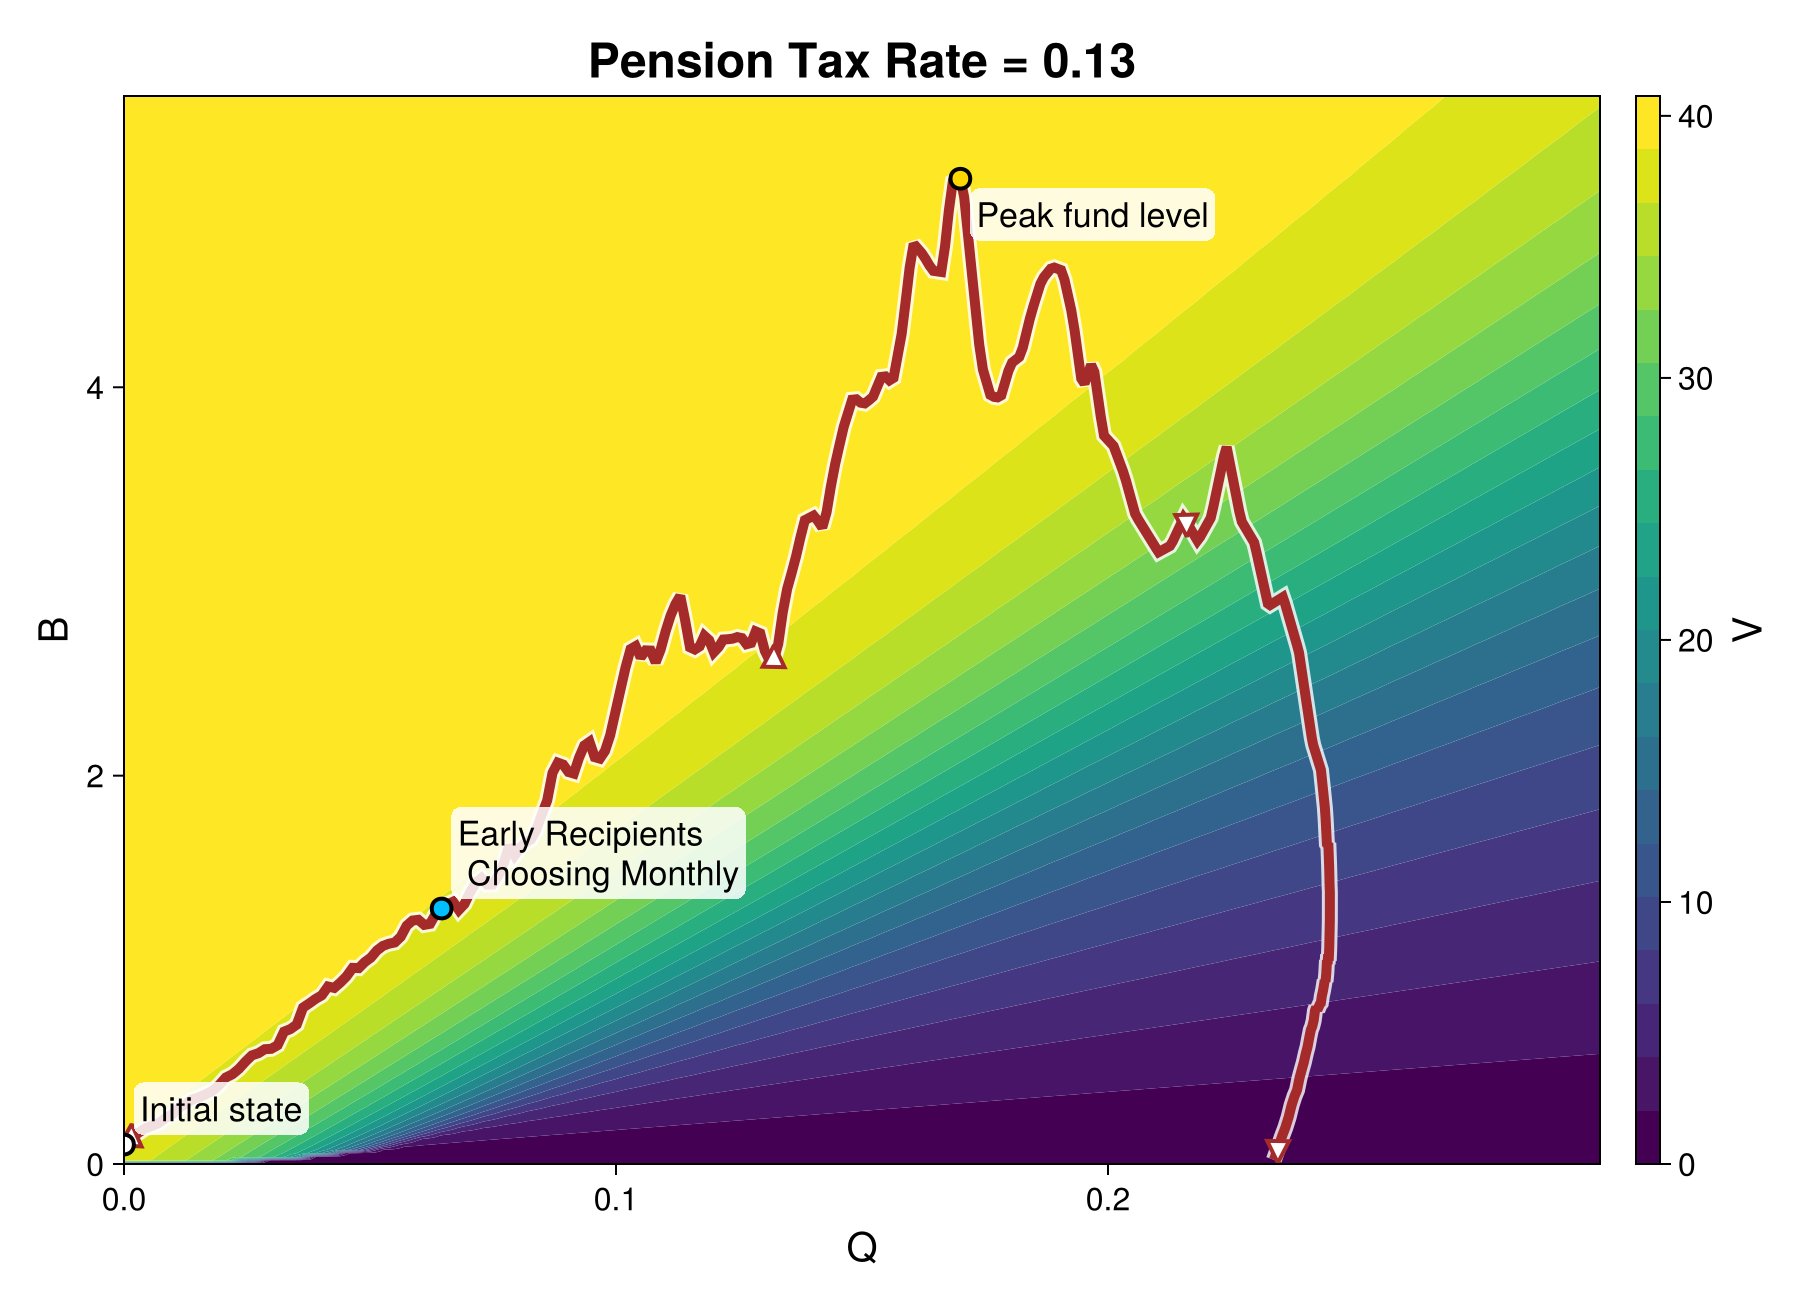
\includegraphics[scale=0.45]{../figure/mechanism_tax_013_stage_3_peak_fund_level.png}}
    \only<5>{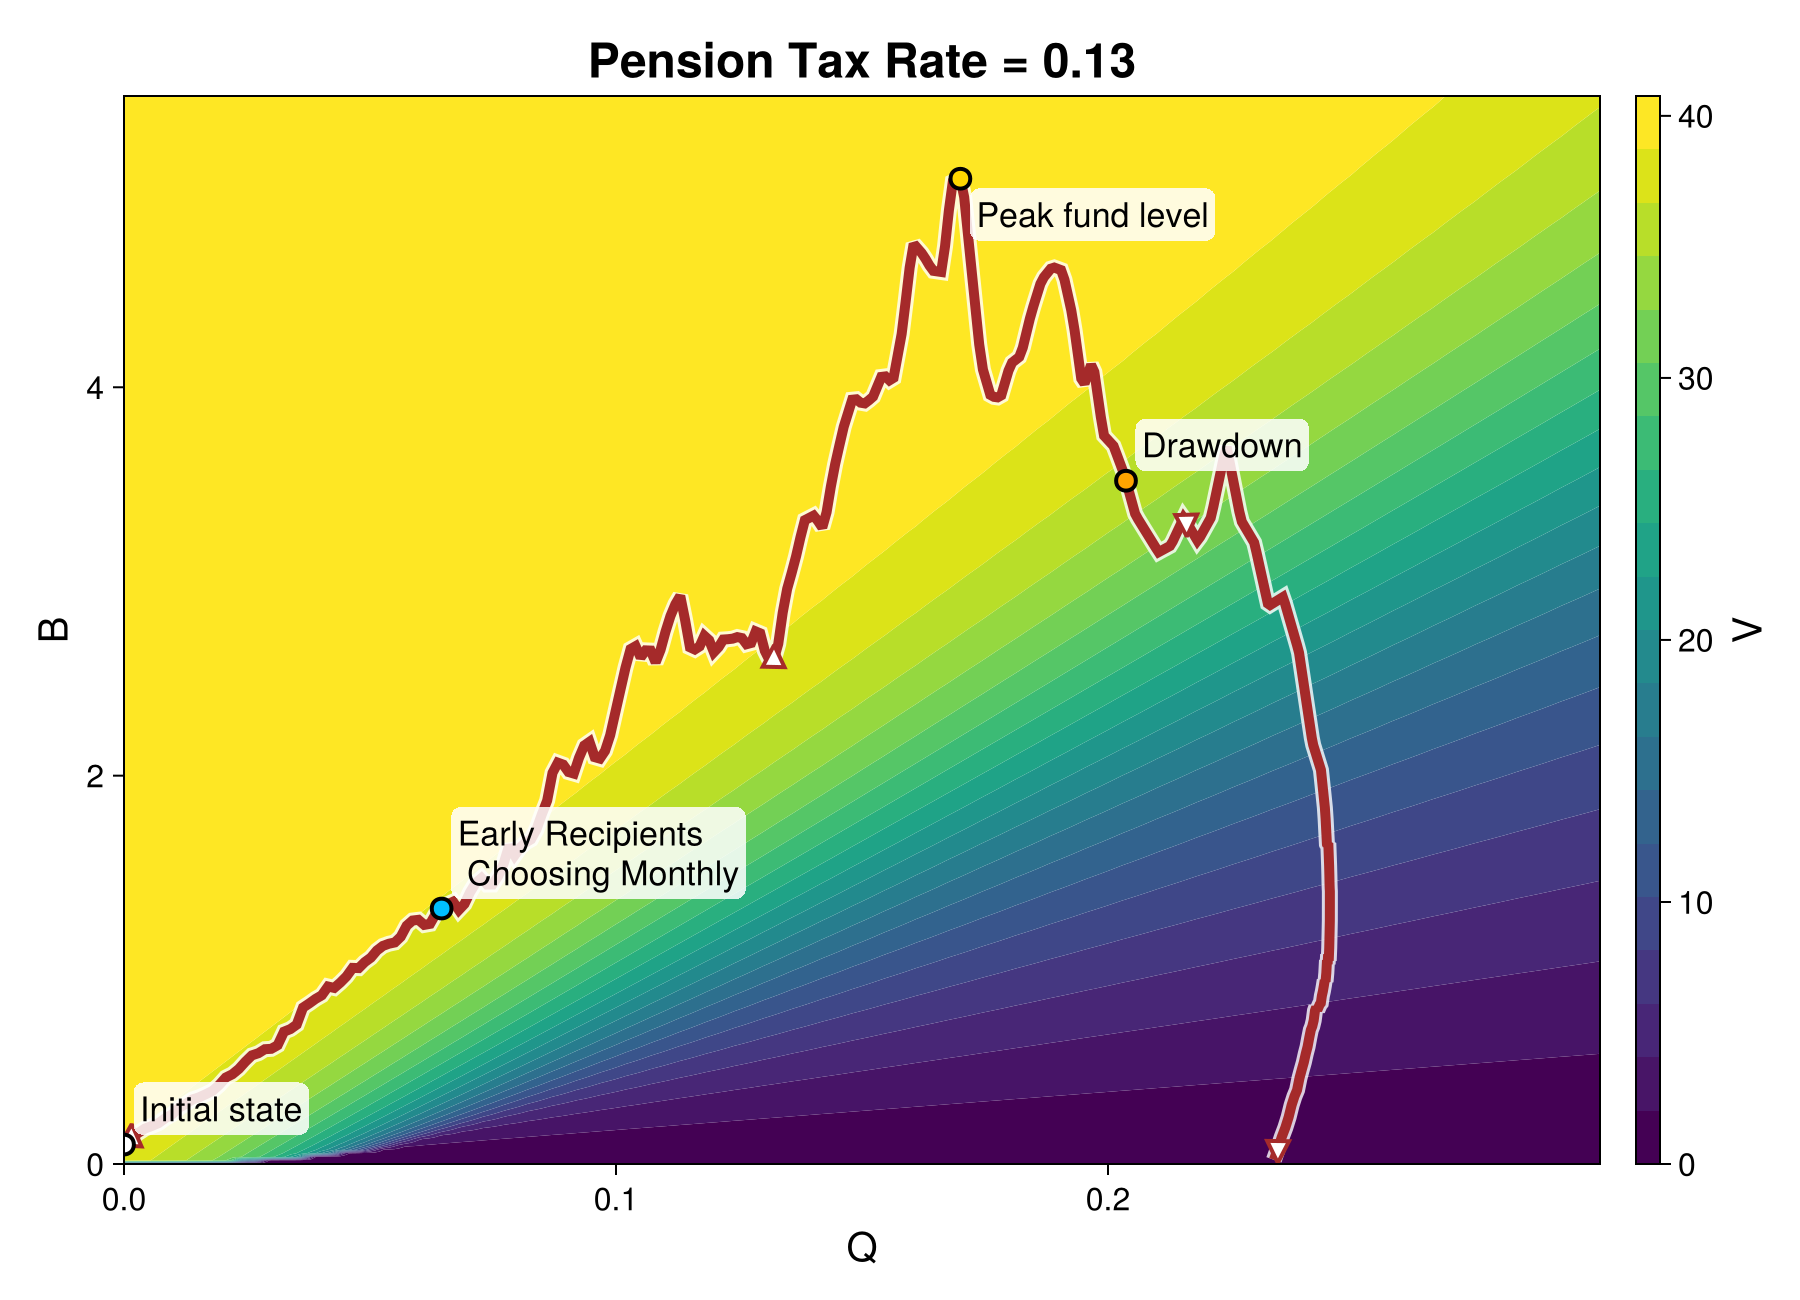
\includegraphics[scale=0.45]{../figure/mechanism_tax_013_stage_4_drawdown.png}}
    \only<6>{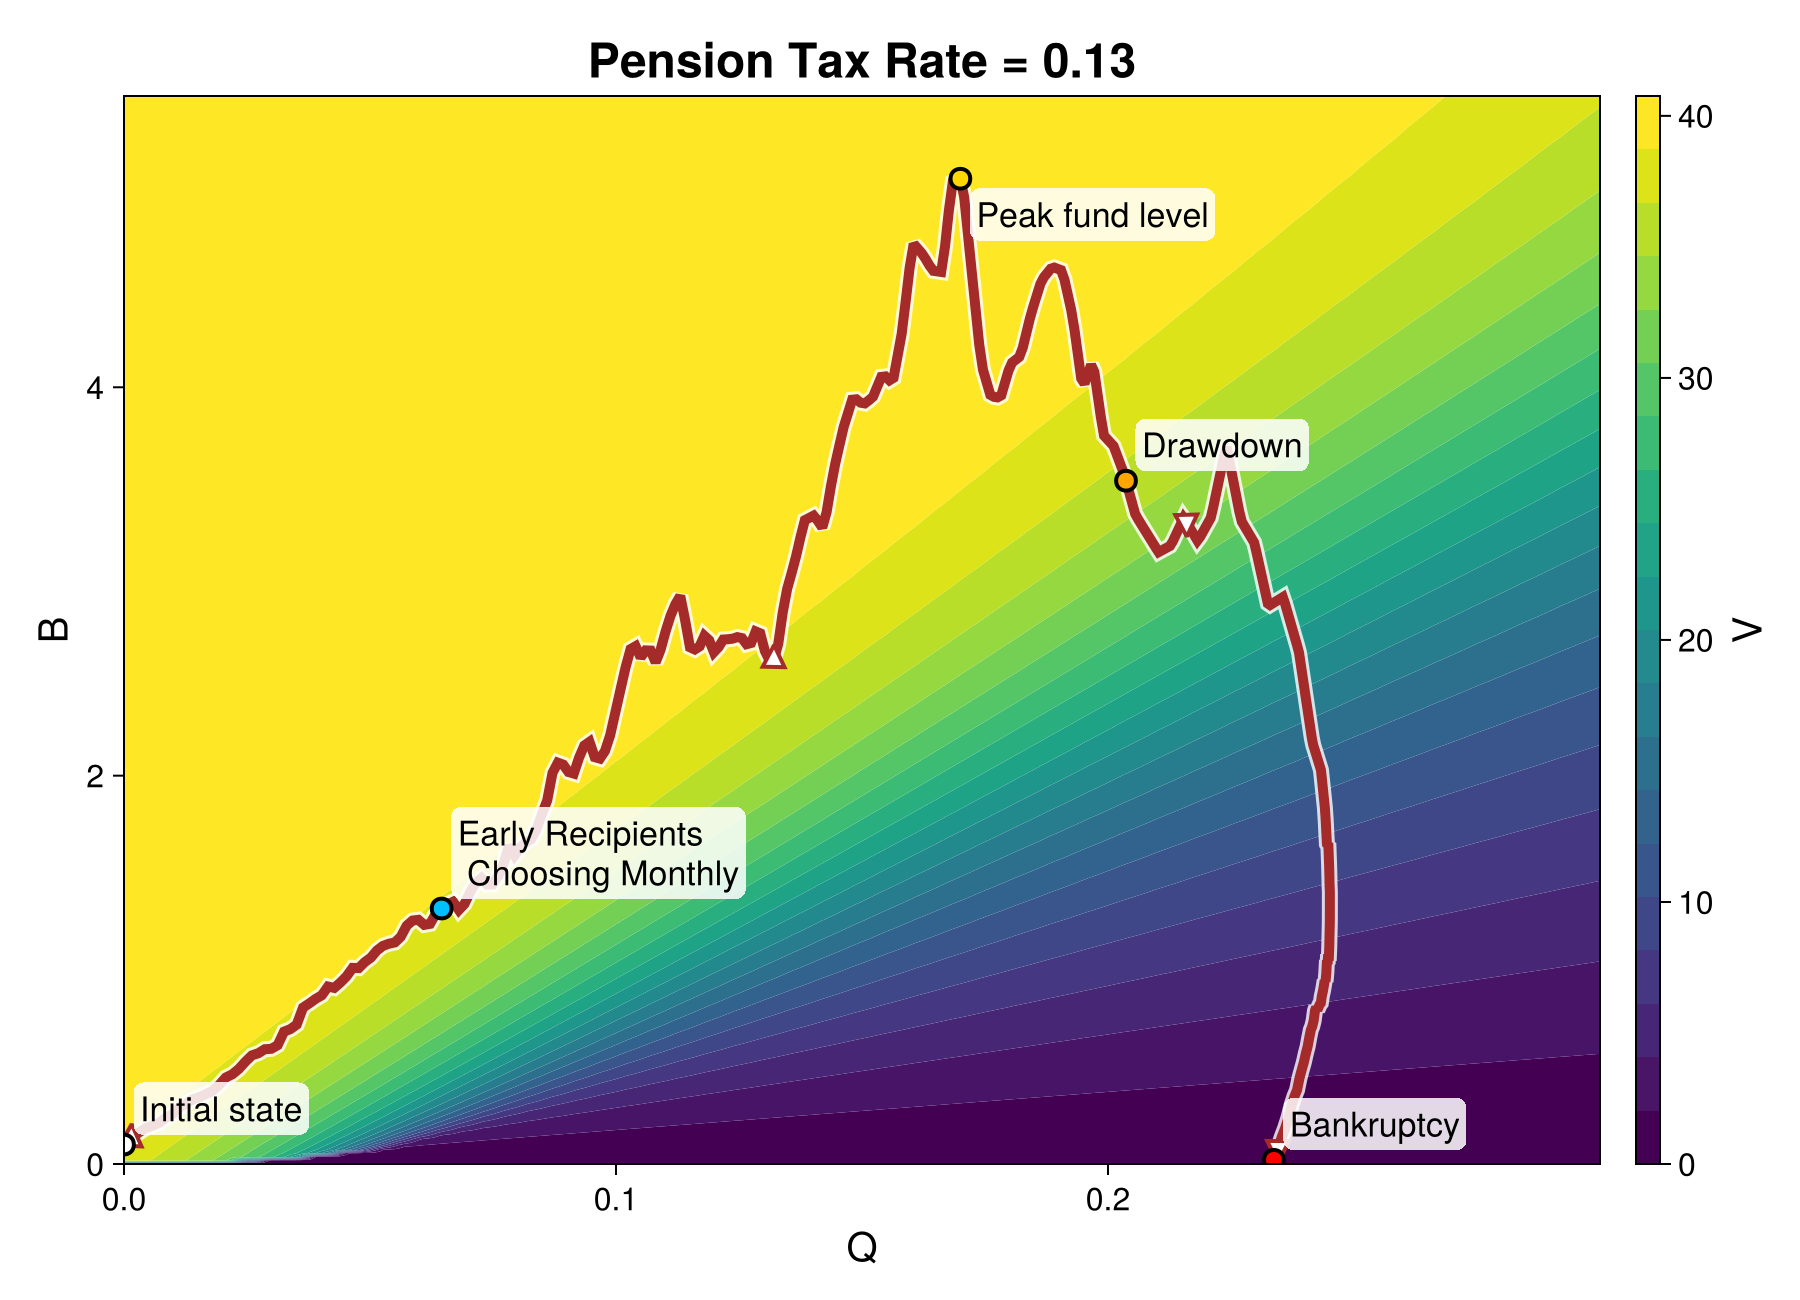
\includegraphics[scale=0.45]{../figure/mechanism_tax_013_stage_5_bankruptcy.png}}
\end{frame}

\begin{frame}{Wrap up}
    \begin{itemize}[<+->]
        \item Low pension tax rate: 
        \begin{itemize}[<+->]
            \item[-] Weak fundamental \\
            \uncover<+->{$\longrightarrow$ Bankruptcy time $\downarrow$} \\
            \uncover<+->{$\longrightarrow$ Fraction of monthly $\downarrow$} \\
            \uncover<+->{$\longrightarrow$ Bankruptcy time $\downarrow$.}
        \end{itemize}
        \item Medium pension tax rate: 
        \begin{itemize}[<+->]
            \item[-] Stronger fundamental \\
            \uncover<+->{$\longrightarrow$ Bankruptcy time $\uparrow$} \\
            \uncover<+->{$\longrightarrow$ Fraction of monthly $\uparrow$} \\
            \uncover<+->{$\longrightarrow$ Fund level $\uparrow$ + Monthly recipients $\uparrow$} \\
            \uncover<+->{$\longrightarrow$ When too many monthly recipients, fund level $\downarrow\downarrow$} \\ 
            \uncover<+->{$\longrightarrow$ Fraction of monthly $\downarrow$ + Many monthly recipients} \\ 
            \uncover<+->{$\longrightarrow$ Bankruptcy time $\downarrow\downarrow$.}
        \end{itemize}
    \end{itemize}
\end{frame}

\begin{frame}{Counterfactuals}
    \begin{itemize}
        \item Experiments simulated from June 2026.
        \begin{itemize}[<+->]
            \item[-] No monthly option or lumpsum option ($\alpha\to\pm\infty$).
            \item[-] Raise pension tax rate.
            \item[-] Cut benefits.
        \end{itemize}
    \end{itemize}
\end{frame}

\begin{frame}{Bankruptcy Probabilities}
    \centering
    \begin{tikzpicture}
        \node[inner sep=0] (simulated-plot) {%
            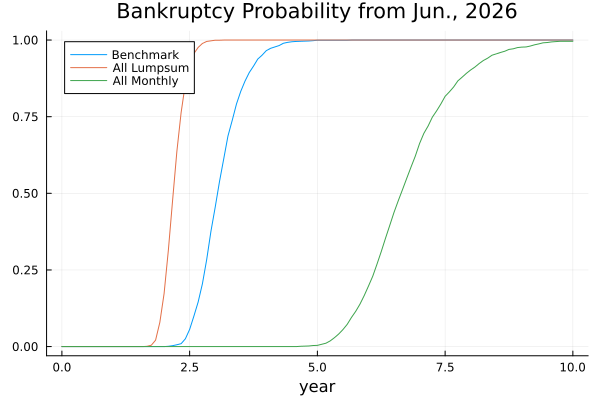
\includegraphics[scale=0.5]{../figure/bankruptcy_prob.png}};
        \only<2>{%
            \node[fill=white, inner sep=1pt] at (simulated-plot.center) {%
                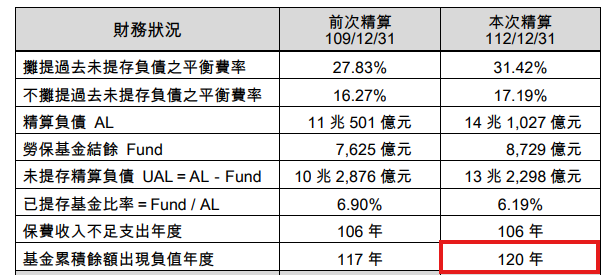
\includegraphics[width=0.8\textwidth]{../figure/LIF_report.png}};}
    \end{tikzpicture}
\end{frame}

\begin{frame}{Bankruptcy Probabilities for Different $\tau$}
    \centering
    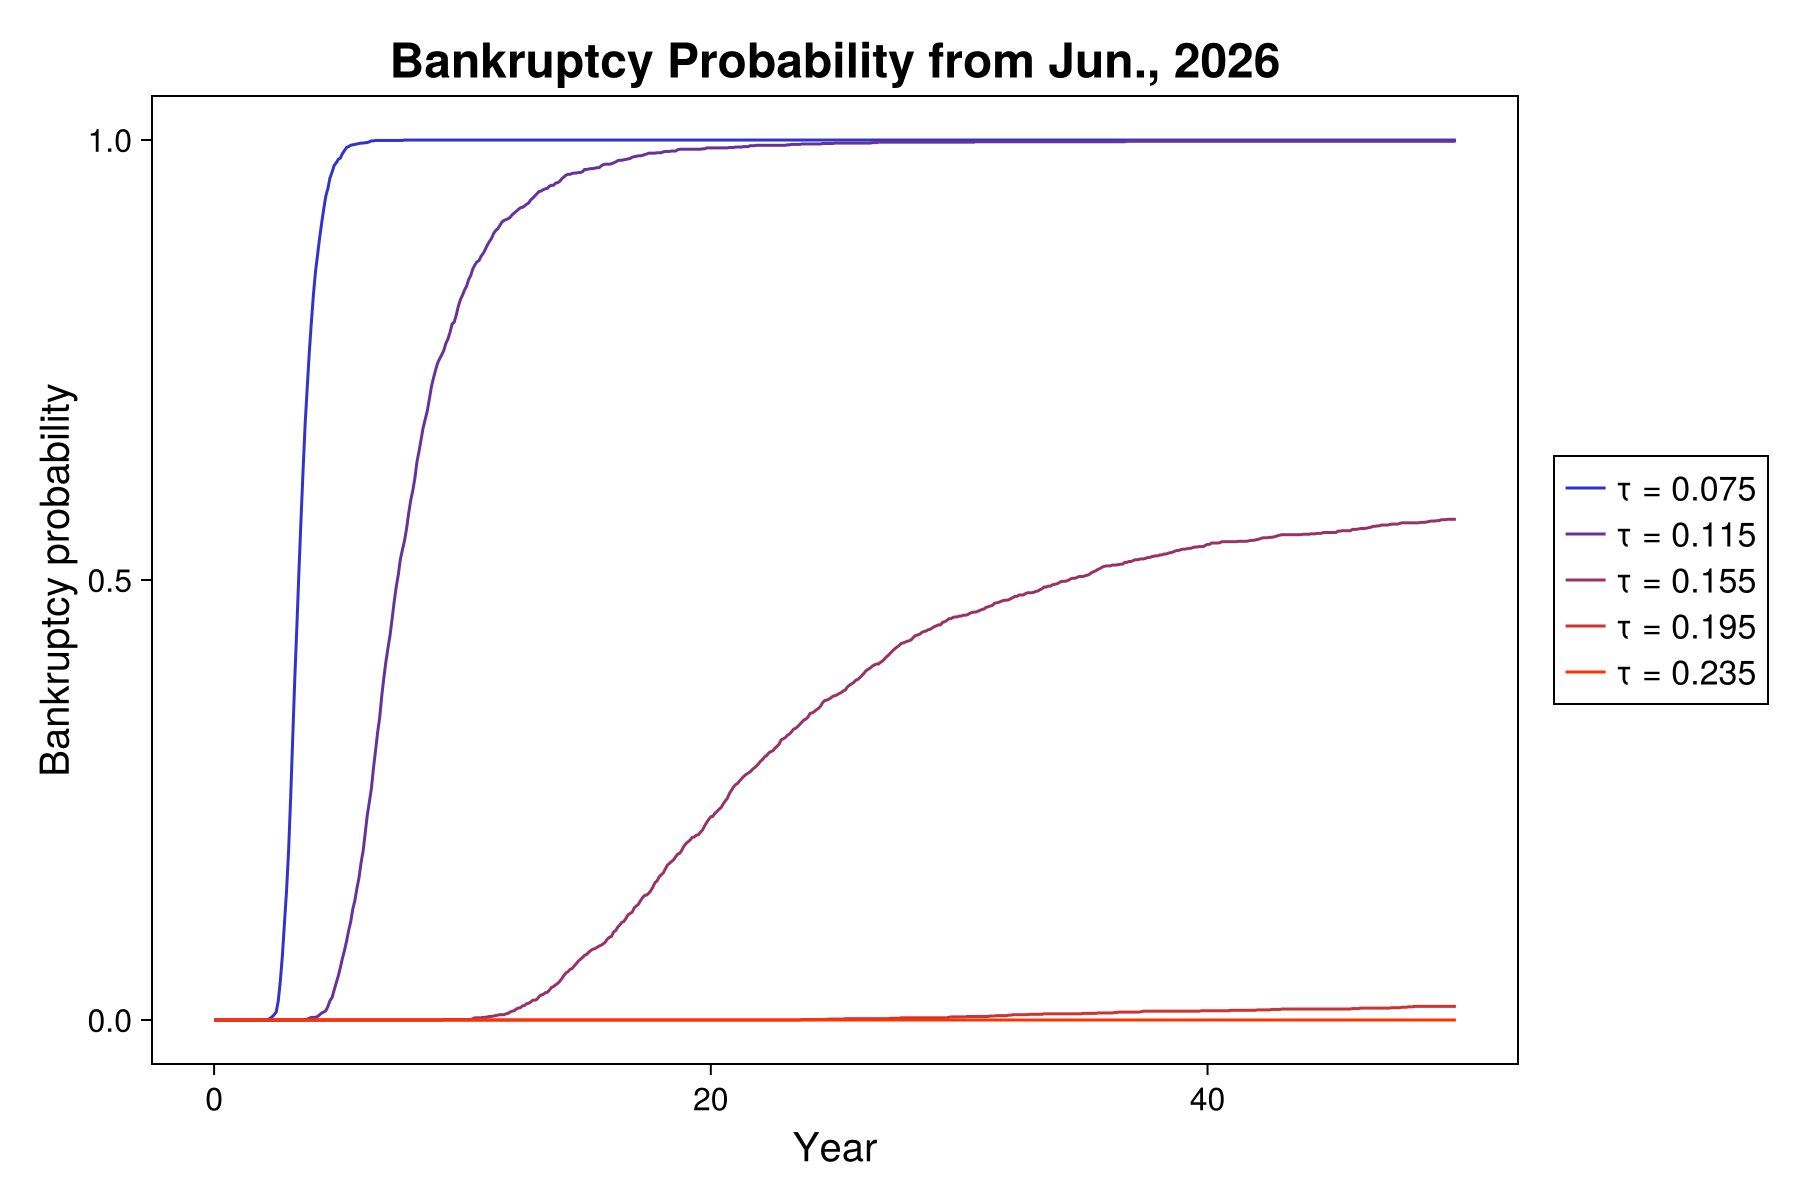
\includegraphics[scale=0.5]{../figure/bankruptcy_prob_tax.png}
\end{frame}

\begin{frame}{Bankruptcy Probabilities for Cutting Benefits}
    \centering
    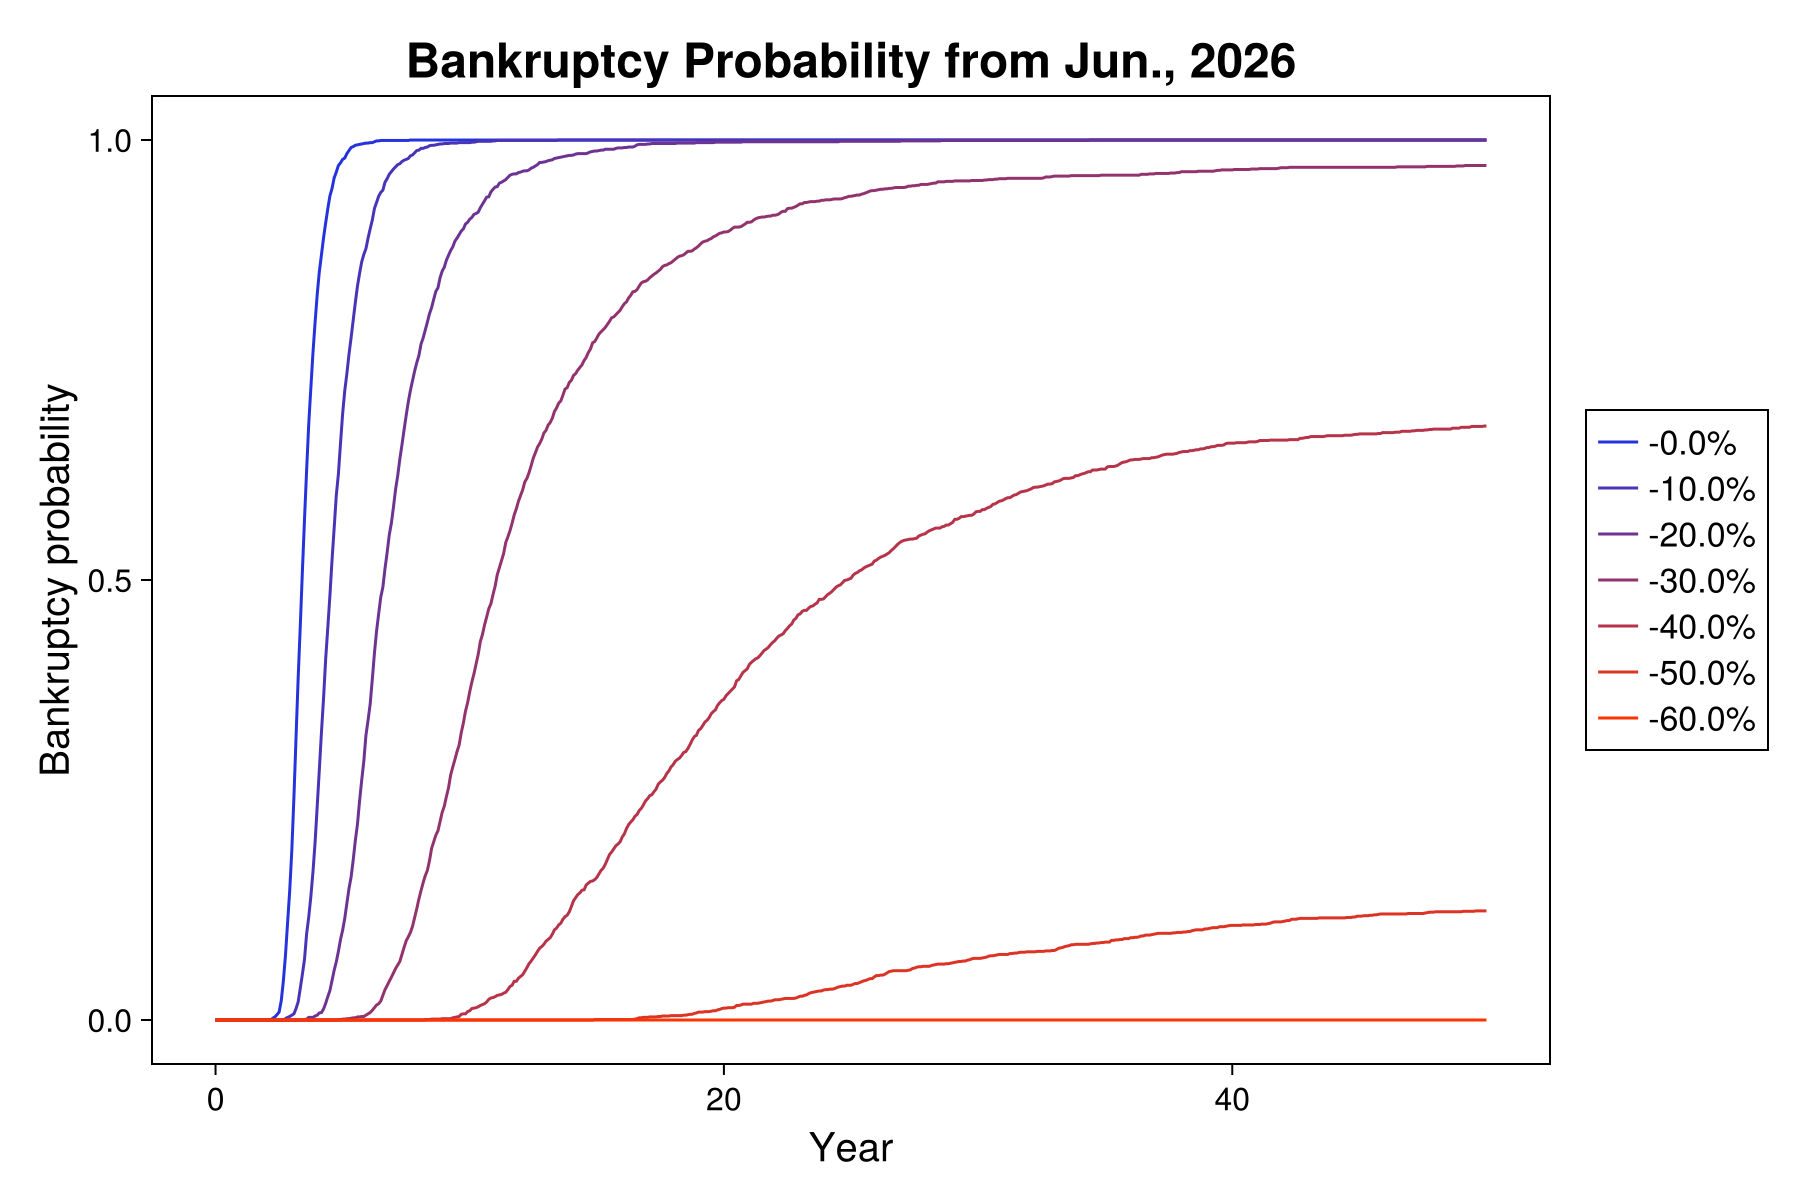
\includegraphics[scale=0.5]{../figure/bankruptcy_prob_cuts.png}
\end{frame}


\begin{frame}{Conclusions}
    \begin{itemize}[<+->]
        \item Take away:
        \begin{itemize}[<+->]
            \item[-] Early recipients are incentivized to take monthly, building up the fragility. 
            \item[-] Lumpsum option accelerates the bankruptcy. 
            \item[-] Raising tax rate to $23.5\%$ or cutting benefits by $60\%$ reduces 
            the bankruptcy probabilities within 50 years near $0$. 
        \end{itemize}
        \item To do:
        \begin{itemize}[<+->]
            \item[-] Relax the mortality assumption. 
            \item[-] Belief on government's reform attitude. 
            \item[-] Endogenous retirement. 
            \item[-] Boom period in return. 
        \end{itemize}
    \end{itemize}
\end{frame}

\section{Appendix}

\begin{frame}[label=data-reconstruction]{Data Explanation}
    \begin{itemize}
        \item \textbf{Official monthly sources (since 2009):}
        \begin{itemize}
            \item[-] Bureau of Labor Funds: fund balance and investment return.
            \item[-] Bureau of Labor Insurance: stocks of monthly recipients and
            new lump-sum claims.
            \item[-] Ministry of the Interior: population and mortality at ages 60+.
        \end{itemize}
        \item BLI reports new monthly recipients (first payments) only from May 2022.
        Before then, reconstruct entries from the stock of monthly recipients:
        \begin{equation*}
            \begin{aligned}
                \text{new monthly recipients}
                ={}& \text{change in the recipient stock}
                + \text{estimated deaths} \\
                &+ \text{average correction from the overlap period}.
            \end{aligned}
        \end{equation*}
        Estimated deaths use the monthly mortality rate implied by annual
        mortality among Taiwan residents aged 60+; negative estimates are set to zero.
    \end{itemize}

    \vspace{0.25em}
    \hyperlink{recipient-fraction}{%
        \beamerreturnbutton{Back to recipient fraction}}
\end{frame}

\begin{frame}[label=reconstruction-validation]{Reconstruction Validation}
    \begin{columns}[c,onlytextwidth]
        \begin{column}{0.73\textwidth}
            \centering
            
\includegraphics[height=0.78\textheight,width=\textwidth,keepaspectratio]{%
                ../figure/validate_reconstruction.png}
        \end{column}
        \begin{column}{0.25\textwidth}
            \centering
            \hyperlink{recipient-fraction}{%
                \beamerreturnbutton{Back to recipient fraction}}
        \end{column}
    \end{columns}
\end{frame}

\begin{frame}[label=recipient-data]{Data}
    \begin{columns}[c,onlytextwidth]
        \begin{column}{0.73\textwidth}
            \centering
            
\includegraphics[width=\textwidth,height=0.78\textheight,keepaspectratio]{%
                ../figure/recipients.png}
        \end{column}
        \begin{column}{0.25\textwidth}
            \centering
            \hyperlink{recipient-fraction}{%
                \beamerreturnbutton{Back to recipient fraction}}
        \end{column}
    \end{columns}
\end{frame}

\begin{frame}[label=state-data]{Data}
    \begin{columns}[c,onlytextwidth]
        \begin{column}{0.73\textwidth}
            \centering
            
\includegraphics[width=\textwidth,height=0.78\textheight,keepaspectratio]{%
                ../figure/state_data.png}
        \end{column}
        \begin{column}{0.25\textwidth}
            \centering
            \hyperlink{recipient-fraction}{%
                \beamerreturnbutton{Back to recipient fraction}}
        \end{column}
    \end{columns}
\end{frame}

\begin{frame}[label=population-density]{Population Density}
    \centering
    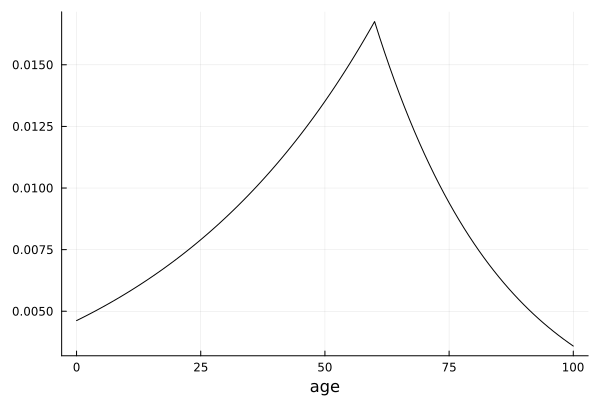
\includegraphics[height=0.78\textheight]{../figure/pop_density.png}

    \vspace{0.25em}
    \hyperlink{population}{\beamerreturnbutton{Back to population}}
\end{frame}

\begin{frame}[label=numerical-algorithm,shrink=15]{Successive Iteration Algorithm}
    \vspace{0.25em}
    \scriptsize
    
\begin{algorithmic}[1]
\Require Initial guess $V^{(0)}$, tolerance $\epsilon>0$, maximum iterations $K$
\State Set $k \gets 0$
\Repeat
    \State Given $V^{(k)}$, compute 
    \begin{equation*}
        \mu_B^{(k)} = \mu_B(B, Q, V^{(k)}(B, Q)), \quad \mu_Q^{(k)} = \mu_Q(B, Q, V^{(k)}(B, Q))
    \end{equation*}
    and the infinitesimal generator 
    \begin{equation*}
        \A^{(k)} = \mu_B^{(k)}\pd{}{B} + \mu_Q^{(k)}\pd{}{Q} + \frac{1}{2}\sigma^2B^2\pdd{}{B}.
    \end{equation*}
    with adjustments to the boundary nodes. 
    \State Solve the linear system 
    \begin{equation*}
        \pth{(\rho+m)I - \A^{(k)}}V^{(k+1)} = \mathbf{b}, \quad 
        \mathbf{b} = p\operatorname{vec}\begin{pmatrix}
            0 & 0 & \cdots & 0 \\ 
            1 & 1 & \cdots & 1 \\ 
            \vdots & \ddots & \ddots & \vdots \\ 
            1 & \cdots & 1 & 1
        \end{pmatrix}.
    \end{equation*}
    \State Compute the error 
    \begin{equation*}
        e^{(k+1)} \gets \norm{V^{(k+1)} - V^{(k)}}_\infty.
    \end{equation*}
    \State $k \gets k+1$
\Until{$e^{(k)}<\epsilon$ or $k=K$}
\State \Return $V^{(k)}$. 
\end{algorithmic}


    \vspace{0.25em}
    \hyperlink{numerical-solution}{\beamerreturnbutton{Back to numerical solution}}
\end{frame}

% \begin{frame}<0>[allowframebreaks]{References}
%    \bibliographystyle{apacite}
%    \bibliography{pension}
% \end{frame}

\end{document}
